%
%
\documentclass{article}
\usepackage{amsmath}
\usepackage{amsthm}
\usepackage{empheq}
\usepackage{graphicx}
\usepackage{bm}
\usepackage{framed}
\usepackage{enumerate}
\usepackage{array}
%\usepackage{pgfplots}
\usepackage{caption}
\usepackage{amsfonts}
\usepackage[margin=3cm]{geometry}
\usepackage{float}

\newcommand{\cO}{\mathcal{O}}                               %
\newcommand{\domain}{\mathcal{D}}                           %
\newcommand{\example}{\textbf{Example:}}                    %
\newcommand{\definition}{\textbf{Definition:}}              %
\newcommand{\theorem}{\textbf{Theorem:}}                    %
\newcommand{\corollary}{\textbf{Corollary:}}                %
\newcommand{\lemma}{\textbf{Lemma:}}                        %
\newcommand{\bp}{\bm{\phi}}                                 % These are used a lot!
\newcommand{\bx}{\bm{x}}                                    %
\newcommand{\rtwo}{\mathbb{R}^2}                            %
\newcommand{\xeq}[1] { \dot{\bm{ #1 }} = \bm{f}(\bm{ #1}) } %

\begin{document}

\title{Dynamical Systems}
\author{Course given by Prof. J.Lister \\
\LaTeX\  by Dominic Skinner \\
Dom-Skinner@github.com}
\maketitle
\section*{Introduction}
A dynamical system is a set of equations describing the evolution of a system
with respect to a time-like variable. Usually they are non-linear.
\\
The possible states of the system define the state space/phase space.
\\
\\
\example\   The logistic map
\[ x_{n+1} = \mu x_n ( 1- x_n) \]
For $ 0 \leq \mu \leq 4 $ this describes evolution with respect to a discrete time 
$n$ in a state space $[0,1]$.
\\
\\
\example\   The Lotka-Voltera equations
\begin{align*}
\dot{r} &= r(a - br -cs) \\
\dot{s} &= s(d - er -fs)
\end{align*}
Where \emph{a-f} are positive constants. These describe continous evolution 
in a state space $(r,s) \in [0 , \infty] \times [0, \infty]$ as a model for 
the population of two species competing for the same food supply.
\\
\\
\example\   The non-linear Schr\"odinger equation
\[ i \frac{\partial \Psi}{ \partial t} = \nabla^2 \Psi + |\Psi|^2 \Psi \]
This describes evolution in an infinite dimensional statespace of possible
wavefunctions.
\\
\\
Because the equations are non-linear, it is often impossible to find a complete
set of closed form analytic solutions. Instead, we resort to a mixture of 
geometric and analytic arguments, and aim to say something about the generic
long-term behaviour.
\\
\\
\example\   
\begin{align*}
\dot{r} &= r(3 - r -s) \\
\dot{s} &= s(2 - r -s)
\end{align*}
Consider the regions where $\dot{r}$ and $\dot{s}$ are $>0, \; <0, \; =0$. 
\\
If $r,s >0$ then
\begin{align*}
r+s &< 2 \implies \dot{r}, \dot{s} > 0 \\
2 < r+s &< 3 \implies \dot{r} >0 , \; \dot{s} < 0 \\
r+s &> 3 \implies \dot{r}, \dot{s} < 0 \\
\end{align*}
$\dot{r} = 0$ if $r=0$ or $r+s = 3$. \\
$\dot{s} = 0$ if $s=0$ or $r+s = 2$. \\
Therefore $\dot{r} = \dot{s} = 0$ at the fixed points $(0,0), \; (3,0), \; (0,2)$.
This gives the phase portrait/diagram/plane%
\footnote{Phase portrait, phase diagram, phase plane will be used interchangably}
% INCLUDE GRAPHIS HERE
\begin{figure}[H]
\centering
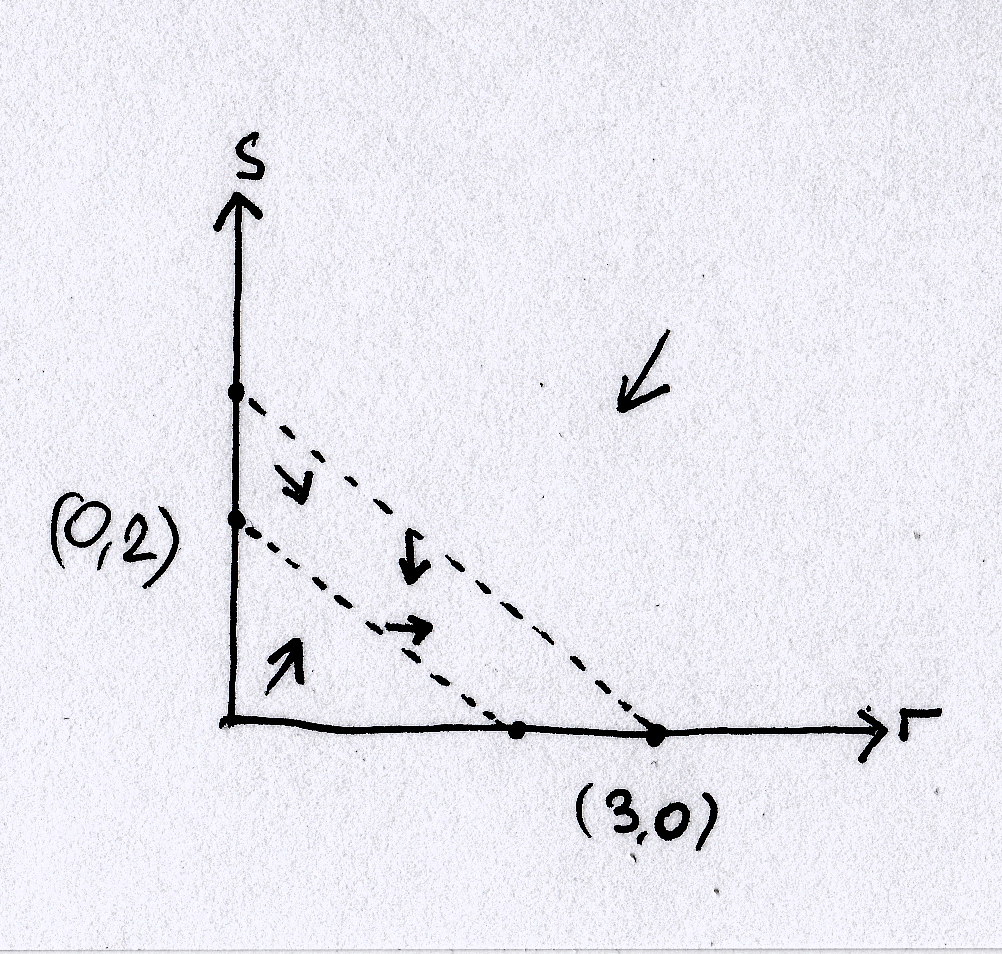
\includegraphics[width=4cm, height=4cm]{fig0.png}
\end{figure}
The most important feature of the phase portrait is that all solutions with 
$r >0$ tend to the stable fixed point $(3,0)$. The fixed points $(0,0)$ and
$(0,2)$ are unstable. There are no periodic orbits.
\\
\\
\example\   
\begin{align*}
\dot{r} &= r(3 - r -s) \\
\dot{s} &= s(2 - \mu r -s)
\end{align*}
In this case, a new fixed point $(\frac{1}{1- \mu} , \frac{2 - 3 \mu}{1- \mu})$
appears in the state space at $\mu = \frac{2}{3}$ and for $\mu < \frac{2}{3}$ 
is the long term stable attractor. 
\\
A qualitative change in the solution structure is called a bifurcation.
\\
\\
\example\   
\begin{align*}
\dot{x} &= -y + \epsilon x (\mu - x^2 - y^2) \\
\dot{y} &= \;\;\; x + \epsilon y (\mu - x^2 - y^2)
\end{align*}
Use polar coordinates which are a more natural choice for this problem.
In general:
\begin{empheq}[box=\fbox]{align}
\dot{r} &= \frac{x \dot{x} + y \dot{y}}{r} \nonumber \\
\dot{\theta} &= \frac{x \dot{y} - y \dot{x} }{ r^2} \nonumber
\end{empheq}
Which are equations that will be referred to frequently. \footnote{so learn them now!}
In our example, they become
\begin{align*}
\dot{r} &= \epsilon r (\mu - r^2) \\
\dot{\theta} &= 1
\end{align*}
Consider $\dot{r}$ and $\dot{\theta}$:
% INSERT DIAGRAM HERE
\begin{figure}[H]
\centering
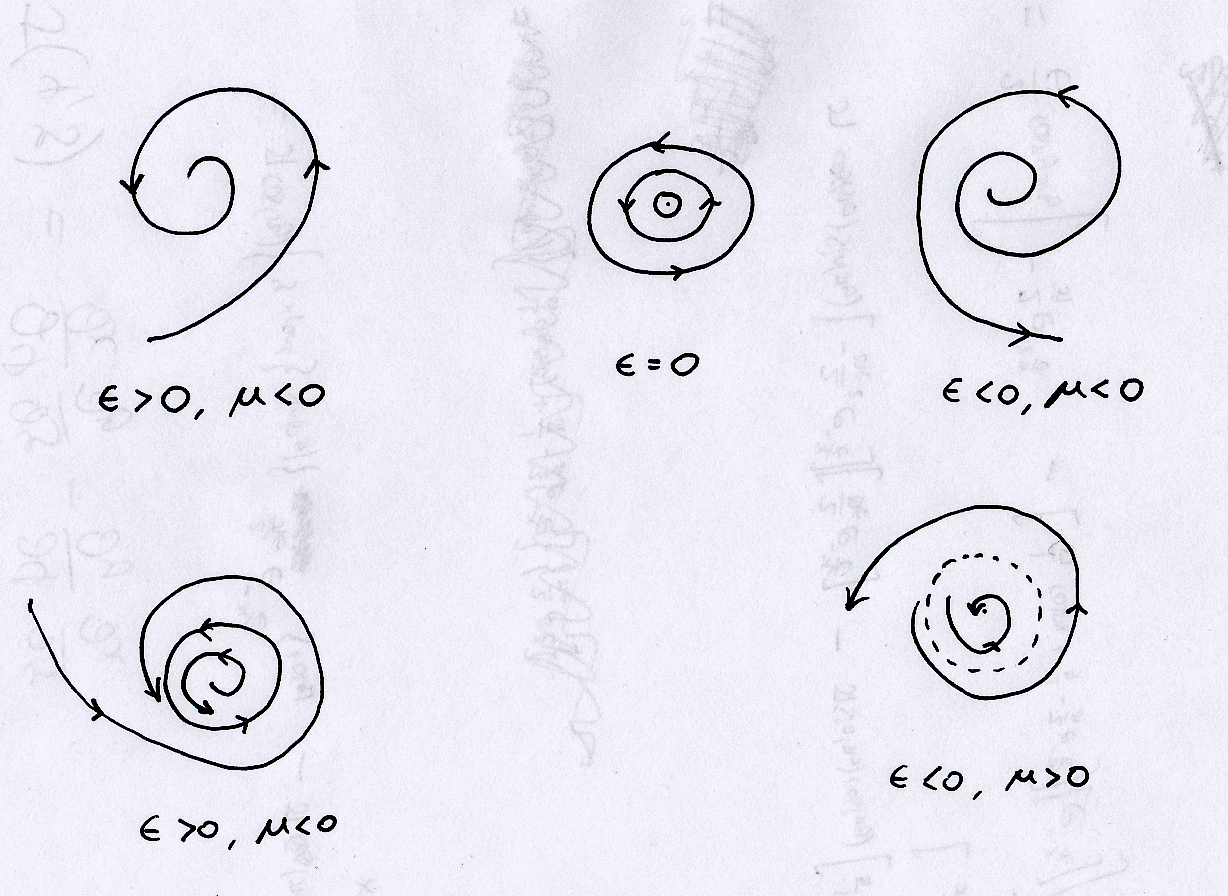
\includegraphics[width=8cm, height=6cm]{fig1.png}
\end{figure}
The infinite set of periodic solutions for $\epsilon = 0$ is destroyed by any 
perturbation to $\epsilon \neq 0$. This is an example of structural instability.
If $\mu > 0$ then just one limit cycle survives and is stable (unstable) for 
$\epsilon >0$ ($\epsilon < 0$). The appearance of the limit cycle as $\mu \uparrow$ 
through $0$ is another form of bifurcation.
\\
\\
\example\ In 2D the points of successive interection $x_n$ of a 
solution near a limit cycle with a line $\varepsilon$ perpendicular to the cycle,
move monotonically towards/away from the point of intersection $x^{*}$ of 
$\varepsilon$ with the limit cycle.
% INSERT PLOT HERE
\begin{figure}[H]
\centering
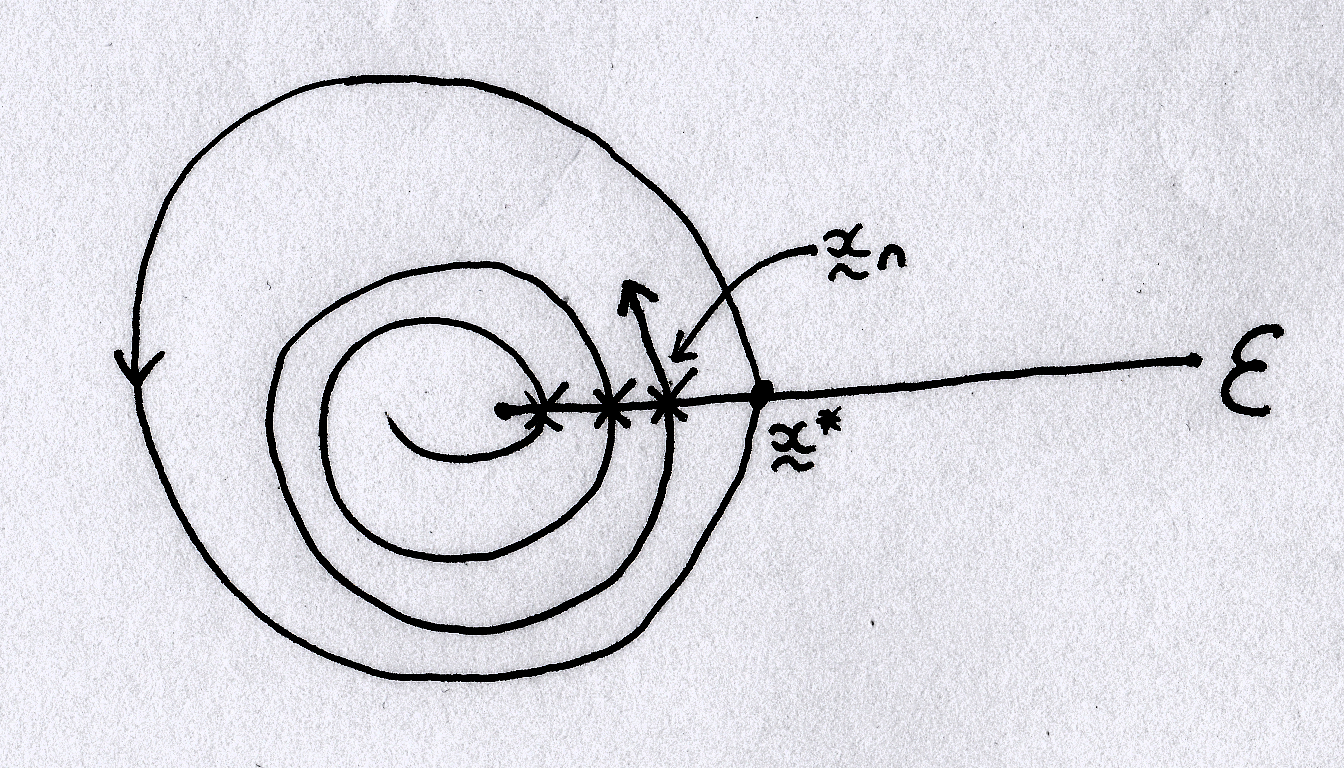
\includegraphics[width=7cm, height=4cm]{fig2.png}
\end{figure}
The point $x^{*}$ is a stable/unstable fixed point of this Poincar\'e recurrence
map.
\\
In 3 or higher dimensions, or in 2D with time-dependent coefficients there is 
room for much more complicated behaviour including \underline{chaos}.
%%%%%%%%%%%%%CHAPTER 1
\section{Basic Definitions}
We need some termonology.
\subsection{Notation}
We only consider ODEs of the form 
\begin{equation}\tag{*}
\xeq{x}
\end{equation}
for \textbf{x} in a phase space/state space $E \subset \mathbb{R}^{n}$.
The n first order ODEs form a dynamical system of order (dimension) n.
\\
\\
Since
\[ \frac{\partial \textbf{f} } { \partial t} = 0 \]
 we call the system \underline{autonomous}.
\\
\\
A non-autonomous system $\dot{\textbf{x}} = \textbf{f}(\textbf{x} ,t) $ can be
made autonomous by setting
\[ \textbf{y} = ( \textbf{x},t) \quad \mbox{ with } \quad \dot{\textbf{y}} = ( \textbf{f}(\textbf{y}),1) \]
The n$^{th}$ order ODE
\[ \frac{d ^n x}{d t^n} = g \left( x , \frac{d x}{d t} , \dots , \frac{d^{n-1} x}{d t^{n-1}} \right) \]
can be put in the form (*) by setting
\[ \textbf{y} =  \left( x , \frac{d x}{d t} , \dots , \frac{d^{n-1} x}{d t^{n-1}} \right) \]
with 
\[ \dot{\textbf{y}} =  \left( y_2 , y_3 , \dots , g( \textbf{y}) \right) \]
Similarly we will consider maps in the form
\[ \textbf{x}_{n+1} = \textbf{F}(\textbf{x}_n) \]
\subsection{Initial Value Problem}
Consider the IVP: 
\[ \dot{\textbf{x}} = \textbf{f}(\textbf{x})  \]
\[ \textbf{x}(t_0)  = \textbf{x}_0\]
In Analysis II we showed that if $\textbf{f}$ satisfies a Lipshitz condition
then we are guaranteed that a solution exists in a neighbourhood of $\textbf{x}_0$,
$ t_0$ and is unique.
\\
(Lipshitz condition is that $\exists$ $L$, $a$, s.t. 
$|\textbf{f}(\textbf{x})- \textbf{f}(\textbf{x})| < L|\textbf{x} - \textbf{y}|$
$, \quad \forall \; |\textbf{x}-\textbf{x}_0|, \; |\textbf{y}-\textbf{x}_0| < a$.)
\\
\\
Moreover, solutions $\textbf{x}(t \, ; \textbf{x}')$ to 
\[ \dot{\textbf{x}} = \textbf{f}(\textbf{x})  \]
\[ \textbf{x}(t_0)  = \textbf{x}'\]
exist, are unique and they depend continously on $\textbf{x}' , \, t$.
\\
\\
Note we are not guaranteed existence for all times.
\\
\\
\example\ 
\[ \dot{x} = x^2  \]
\[ x(0)  = 1\]
This has solution
\[ x(t) = \frac{1}{1-t} \]
and so $x \to \infty$ as $t \uparrow 1$.
\\
\\
If $|\textbf{x}(t)| \to \infty$ as $t \to T \;(< \infty)$ then we call this
finite time blow up.
\\
\\
\example\ Non-uniqueness when $\textbf{f}$ is non-Lipshitz. If
\[ \dot{x} = \left\{\begin{array}{lr}
				\sqrt{x} & \mbox{for } x >0 \\
				0        & \mbox{for } x \leq 0
				\end{array}
\right. \mbox{ and } x(0) = 0 \]
Then there is a family of solutions
\[ \left. \begin{array}{lr} 
				x = 0 & t < \tau \\
				x = \frac{1}{4}(t - \tau)^2 & t > \tau
\end{array} \right\} \mbox{ for any } \tau \geq 0 \]
From now on we will assume that \textbf{f} is differentiable ( and so Lipshitz).
\\
\subsection{Trajectories and Flows}
Consider the autonomous system
$ \dot{\textbf{x}} = \textbf{f}(\textbf{x}) $
The solution $\textbf{x}(t)$ to the IVP with $\textbf{x}(0) = \textbf{x}_0$
defines a trajectory. (orbit/integral curve)
\\
\\
The distance travelled along this curve clearly only depends on $t - t_0$, 
and we could consider lots of starting points $\textbf{x}_0$.
\\
This motivates the idea of a flow. 
\\
\\
\definition\ (Flow) \\
Given \textbf{f}, the corresponding flow is defined to be a (the) function
$\bp_t (\textbf{x}) $ from $E \times \mathbb{R} \to E$ such that
\[ 
\frac{\partial}{\partial t} \bp_t ( \bm{x} ) = \bm{f}(\bp_t (\bm{x} ) ), \qquad\
\bp_0(\bm{x}) = \bm{x} 
 \]
The solution to the IVP $\dot{\bm{x}} = \bm{f}(\bm{x}), \; \bm{x}(t_0) = \bm{x}_0$,
is just $\bm{x}(t) = \bp_{t - t_0} (\bm{x}_0)$
\\
Clearly 
\[ \bp_{s+t}(\bm{x}) = \bp_s(\bp_t(\bm{x})) = \bp_t ( \bp_s (\bm{x} ) ) \]
\begin{framed}
\noindent Aside: We can establish another link with maps, by defining 
$\bm{x}_{n+1} = \bm{F}(\bm{x}_n) = \bp_{\Delta t} (\bm{x}_n)$. \\
Clearly $\bp_{n \Delta t} (\bm{x} ) = \bm{F} ( \bp_{(n-1) \Delta t} (\bm{x} )) = \bm{F}^n(\bm{x}) $ 
\end{framed}
\subsection{Flows, Trajectories, Orbits, Invariant Sets, \& Limiting Sets}
Using the idea of a flow, we define the following:
\\
\\
\definition\ Orbits/Trajectories
\\
 The orbit of $\bp_t(\bm{x})$ through $\bm{x}_0$ is
the set $\cO(\bm{x}_0) = \{ \bp_t(\bm{x}_0): -\infty < t < \infty \}$.
\\
The forwards (backwards) orbit is 
\[\cO^{+ \, (-)}(\bm{x}_0) = \{ \bp_t(\bm{x}_0):  t \geq 0 \; (t \leq 0) \} \]
\definition\ Invariant sets
\\
A set of points $\Lambda \subset E$ is invariant if
$\bm{x} \in \Lambda \implies \cO(\bm{x}) \subset \Lambda$
\\
Clearly $\cO(\bm{x}_0)$ is invariant, and so is any union of orbits.
\\
\\
Particular cases of interest are
\\
\\
\definition\ Fixed points
\\
$\bm{x}_0$ is a periodic point with period $T$ if $\bp_T(\bm{x}_0)= \bm{x}_0$
for some $T>0$ and $\bp_t (\bm{x}_0) \neq \bm{x}_0$ for $0 < t < T$.
The set $ \{ \bp_t ( \bm{x}_0) : 0 \leq t < T \}$ is the periodic orbit
through $\bm{x}_0$.
\\
\\
\definition\ Limit Cycle
\\
A limit cycle is an isolated periodic orbit, i.e. there are no other periodic
orbits within a sufficiently small neighbourhood.
\\
\\
\definition\ Homoclinic and Heteroclinic orbits
\\
If $\bm{x}_0$ is a fixed point and $\exists \; \bm{y} \neq \bm{x}_0$ such that
$\bp_t(\bm{y}) \to \bm{x}_0$ as $t \to \pm \infty$ then 
$\cO(\bm{y})$ is a homoclinic orbit.
\\
\\
If $\bm{x}_0$, $\bm{x}_1$ are fixed points and 
$\exists \; \bm{y} \neq \bm{x}_0 , \, \bm{x}_1$ with $\bp_t (\bm{y}) \to \bm{x}_0$
as $t \to - \infty$, $\bp_t(\bm{y}) \to \bm{x}_1$ as $t \to + \infty$ then
$\cO(\bm{y})$ is a heteroclinic orbit.
%
\begin{figure}[H]
\centering\caption*{Example of a Heteroclinic and a Homoclinic orbit}
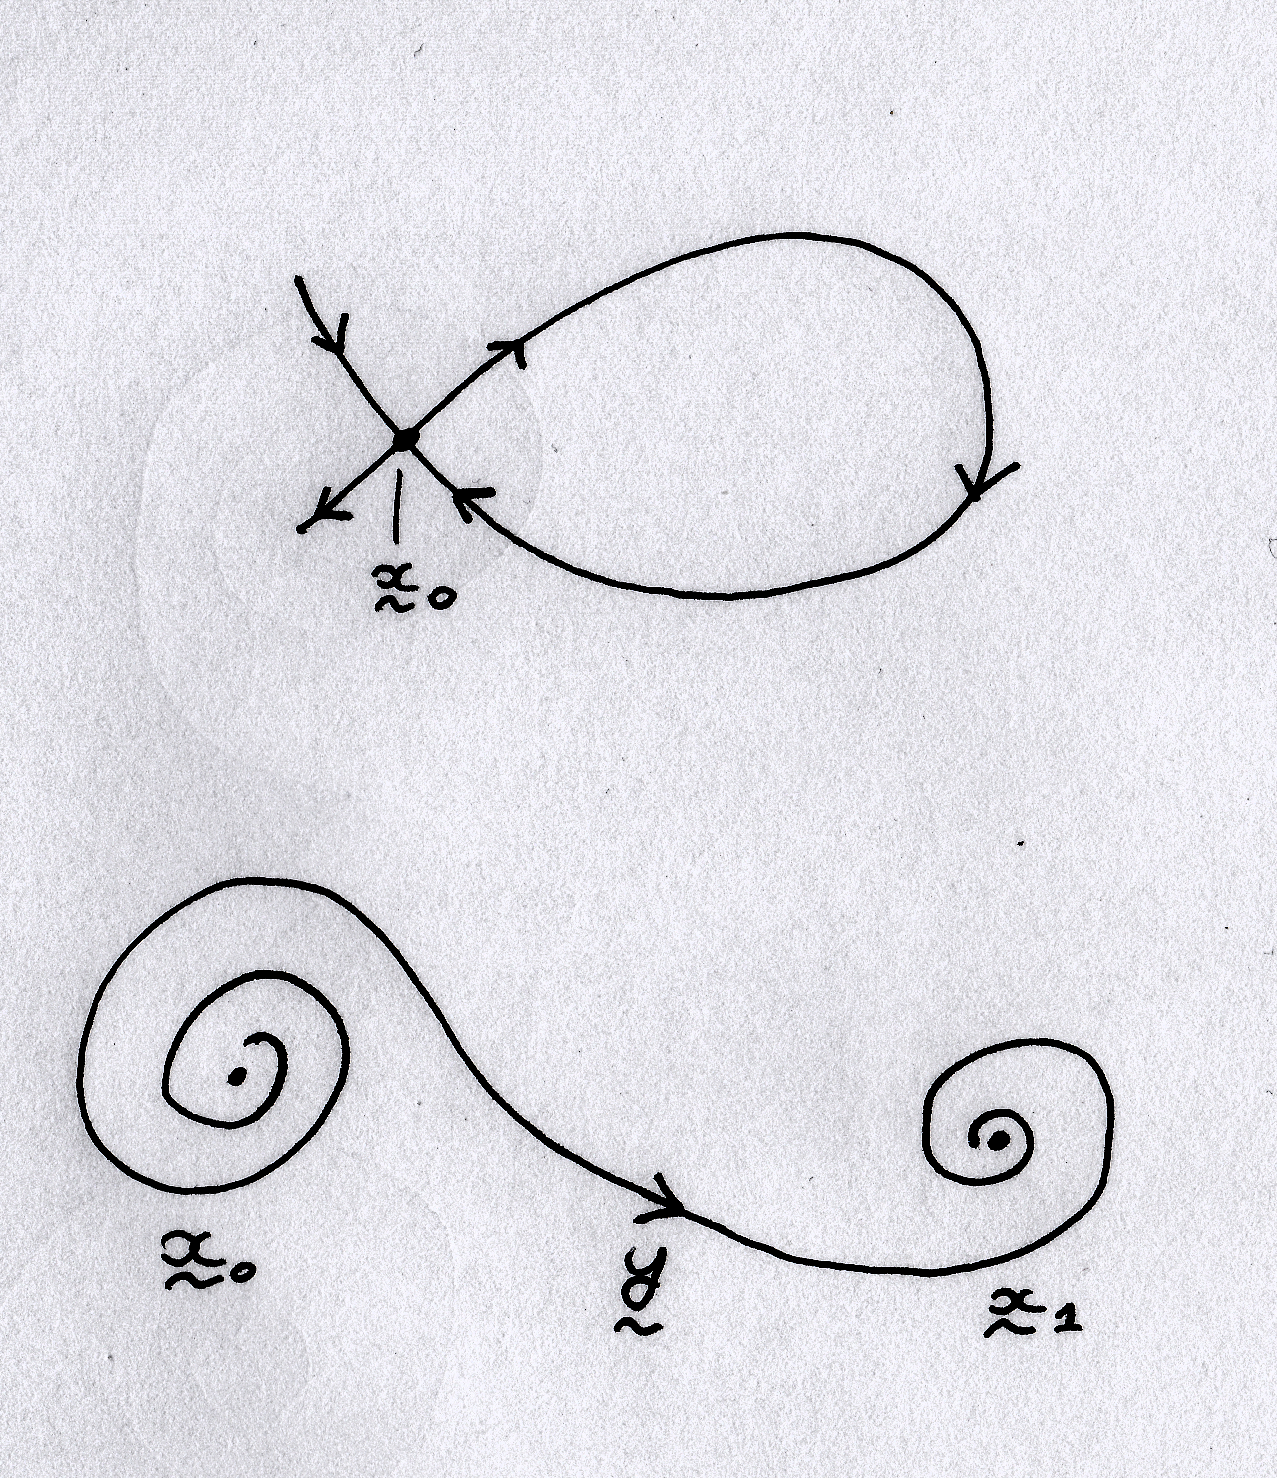
\includegraphics[width=4cm, height=6cm]{fig3.png}
\end{figure}
\noindent If we are interested in the long-term behaviour of trajectories, it is not 
enough simply to think of 
\[ \lim_{t \to \infty} \bp_t(\bm{x}) \]
because the limit might not exist; for example a limit cycle.
\\
\\
\definition\ Limit set
\\
The $\omega$-limit set of $\bm{x}$ is 
\[ \omega (\bm{x}) = \{ \bm{y} : \exists \mbox{ a sequence } (t_n) \mbox{ with }\
 \bp_{t_n}(\bm{x}) \to \bm{y} \mbox{ and } t_n \to \infty \} \]
Similarly the $\alpha$ limit set is defined by sequences with $t_n \to - \infty$.
\\
\\
\example\ \\
%
\begin{center}
\begin{tabular}{ m{4.5cm} m{4.5cm}  }\centering 
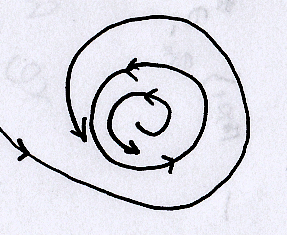
\includegraphics[scale = 0.35]{fig4.png}  & 
$ \begin{array}{rl}
\dot{r} &= r(1-r^2) \\
\dot{\theta} &= 1
 \end{array}$
\end{tabular} 
\end{center}
%
For $\bm{x}$ with $0 < |\bm{x}| < 1$ we have that
\[ \omega ( \bm{x} ) = \{ \bm{y} : |\bm{y}| = 1 \}  \qquad  \alpha ( \bm{x} ) = \{\bm{0} \} \]
For $|\bm{x}|>1$
\[ \omega ( \bm{x} ) = \{ \bm{y} : |\bm{y}| = 1 \}  \qquad  \alpha ( \bm{x} ) = \{ \} \]
\\
\\
In fact, the limit sets are always invariant sets since
\begin{itemize}
\item If $\cO(\bm{x})$ is bounded then $\omega(\bm{x})$ is non-empty.
\item If $\bp_t(\bm{x}) \to \infty$ then $\omega(\bm{x}) = \{ \} $.
\end{itemize}\vspace{3mm}
\definition\ (For maps) 
\\
Fixed points solve $\bm{F}(\bm{x}) = \bm{x}$. Orbits, periodic points etc.
are defined as above by replacing $\bp_t(\bm{x})$ by $\bm{F}^n(\bm{x})$,
etc.
\\
\\
A periodic orbit with period N is called an N-cycle.
\subsection{Topological equivalence and structural stability of flows}
This section is in a handout.
\\
\section{Flow near fixed points}
The simplest features of a flow are the fixed points. Find them by first 
solving $\bm{F}(\bm{x}) = \bm{0}$.
\\
\subsection{Linearisation}
If $\bm{f}$ is sufficiently smooth and $\bm{x}_0$ is a fixed point, we expand
in a Taylor series with $\bm{f}(\bm{x}_0)=\bm{0}$ to obtain 
\[\dot{\bm{y}} = A\bm{y} + O(|\bm{y}|^2)\]
 where $\bm{y} = \bm{x} - \bm{x}_0$ and
\[ A_{ij} = \left. \frac{\partial f_i}{\partial x_j}\right| _{\bm{x}_0}\]
is the Jacobian matrix (Written $D\bm{f}$ in Glendinning).
\\
\\
The hope (see below when it is true) is that the flow $\bp_t^{\bm{f}}$ is
like the flow corresponding to the linearization $\dot{\bm{y}} = A \bm{y}$.
\\
\subsection{Classification of fixed points}
In 2D, 
\[ A = \left( \begin{array}{cc}
		a & b \\
		c & d \end{array} \right) \]
with $D = ad - bc$, $T = a+d$ and the eigenvalues are
\[ \lambda_{1,2} = \frac{1}{2}(T \pm \sqrt{T^2 - 4T}) \]
\begin{enumerate}[(i)]
\item Saddle points ($D<0$, real $\lambda$'s with opposite signs)
\\
\begin{tabular}{ m{5cm} m{3cm} m{3cm}} 
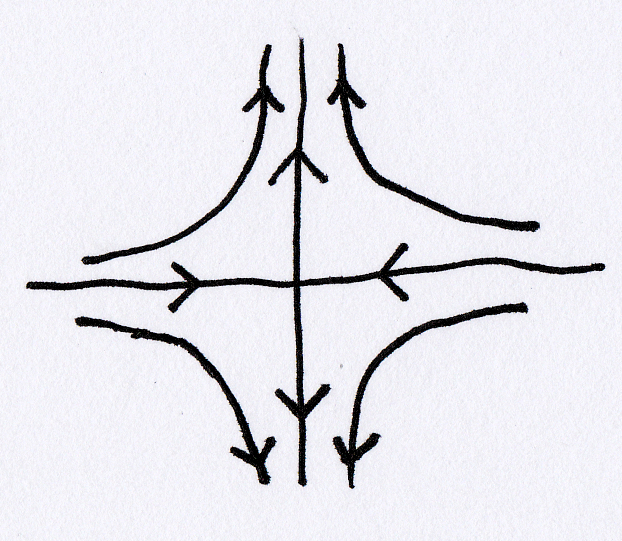
\includegraphics[scale = 0.15]{fig5.png}  & 
 $ A = \left( \begin{array}{cc}
		\lambda _1 &  \\
		 & \lambda _2 \end{array} \right) $ & \makebox[5pt][l]{$ \lambda_1 < 0 <\lambda_2 $} \\
\end{tabular}

\item Stable nodes ($0< 4D < T^2$, $T<0$, real roots, both negative)
\\
\begin{tabular}{ m{3.5cm} m{2cm} m{6cm}} 
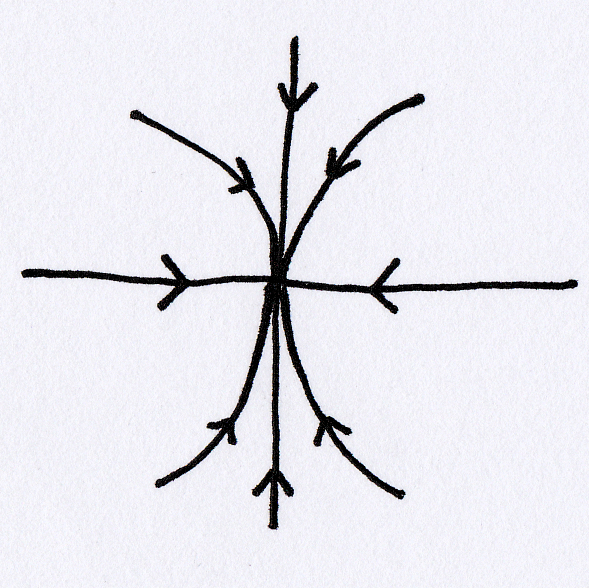
\includegraphics[scale = 0.15]{fig6.png}  & 
$ \lambda_1 < \lambda_2 < 0 $ & $ \frac{y_2}{y_1} \propto \
e^{(\lambda_2-\lambda_1)t} \to \infty \;\; \mbox{as} \;\; t \to \infty $
\end{tabular}

\item Unstable node ($0 < 4D < T^2$, $T>0$, real roots, both positive)
\\
\begin{tabular}{ m{4.5cm} m{2cm} m{6cm}} 
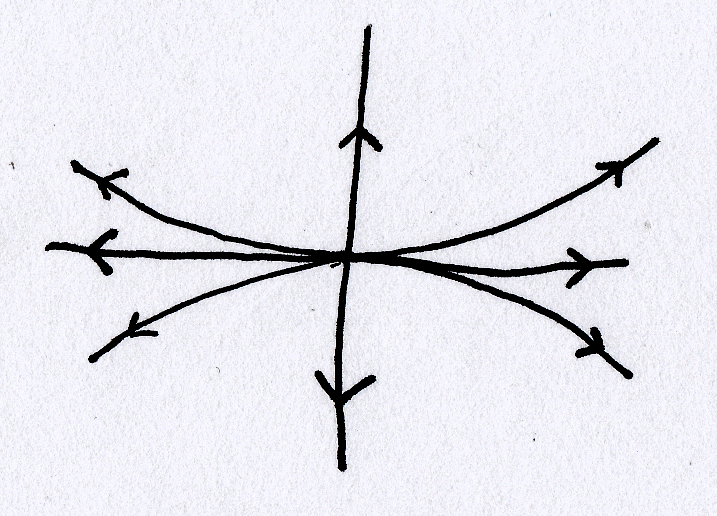
\includegraphics[scale = 0.15]{fig7.png}  & 
$ \lambda_1 < \lambda_2 < 0 $ & $ \frac{y_2}{y_1} \propto \
e^{(\lambda_2-\lambda_1)t} \to 0 \;\; \mbox{as} \;\; t \to -\infty $
\end{tabular}

\item Stable focus ($ T^2 < 4D $, $T<0$, complex roots, 
$\lambda = \rho \pm i \omega$, $\rho < 0$)
\\
\begin{tabular}{ m{5.5cm} m{3cm} m{3cm} } 
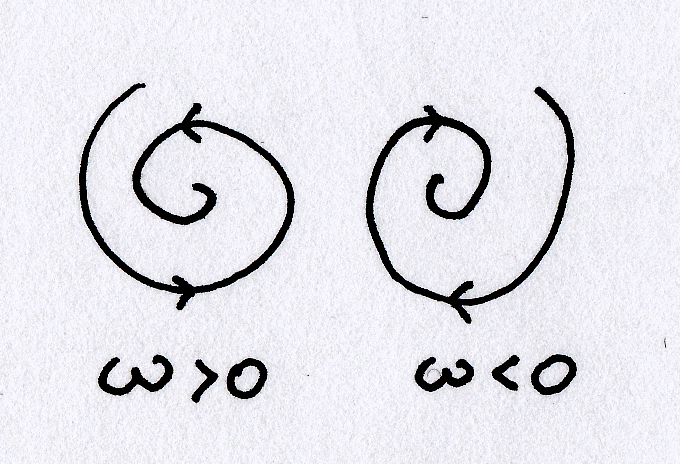
\includegraphics[scale = 0.18]{fig8.png}  & 
$  A = \left( \begin{array}{cc}
		\rho & -\omega \\
		 \omega & \rho \end{array} \right) $
 & $ \dot{r} = \rho r \qquad \dot{\theta} = \omega $
\end{tabular}

\item Unstable focus ($ T^2 < 4D $, $T>0$, complex roots, $\rho > 0$)

\item Two degenerate cases with equal eigenvalues on the border $T^2 = 4D$
between nodes and foci. (e.g. $\lambda > 0$)
\[\begin{array}{c@{\hspace{2cm}}c}
\mbox{Stellar Node} & \mbox{Improper Node} \\ \\
  A = \left( \begin{array}{cc}
		\lambda & 0 \\
		 0 & \lambda \end{array} \right)  & 
  A = \left( \begin{array}{cc}
		\lambda & 1 \\
		 0 & \lambda \end{array} \right)   \\
\end{array}
\]
\begin{center}
\hspace{1mm} 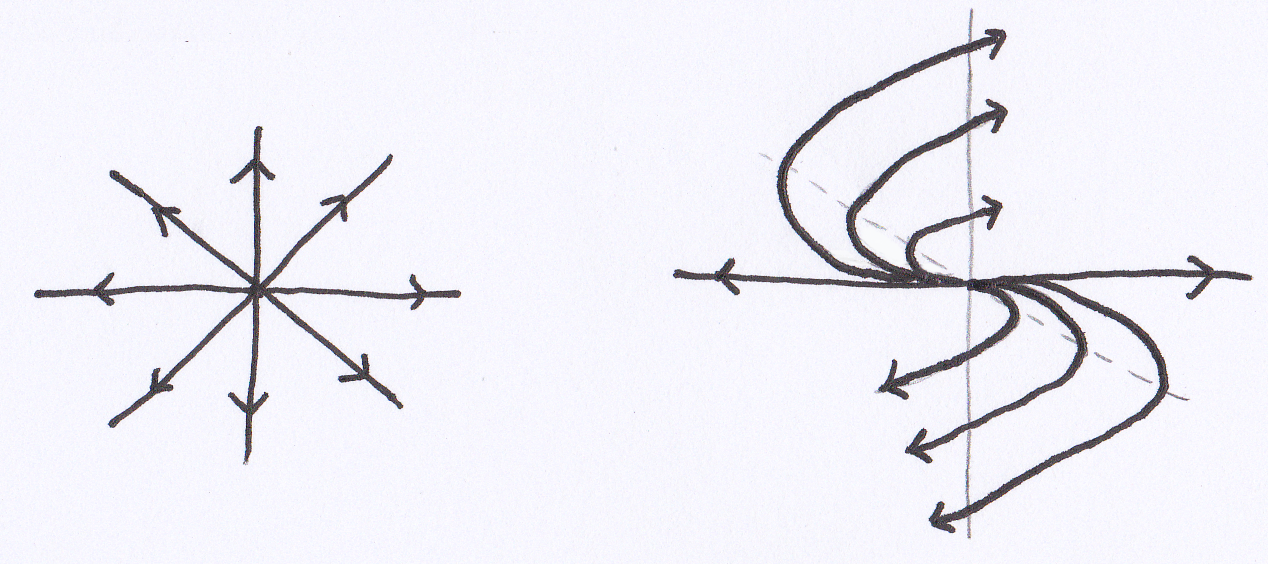
\includegraphics[scale=0.15]{fig95.png}
\end{center}
\item Centres ($T=0$, $D>0$, $\lambda = \pm i \omega$)
\\
\begin{tabular}{ m{4.5cm} m{8cm}  } 
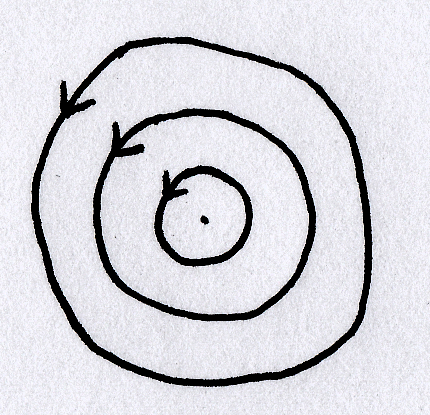
\includegraphics[scale = 0.15]{fig11.png}  & 
All trajectories are closed. This is on the border between stable foci and
unstable foci.
\end{tabular}

\item Line of Fixed points. Specia case on the border $D=0$ between saddles and
nodes, where at least one $\lambda$ is zero. For example, 
\\
\\
\begin{tabular}{ m{4.5cm} m{8cm}  } 
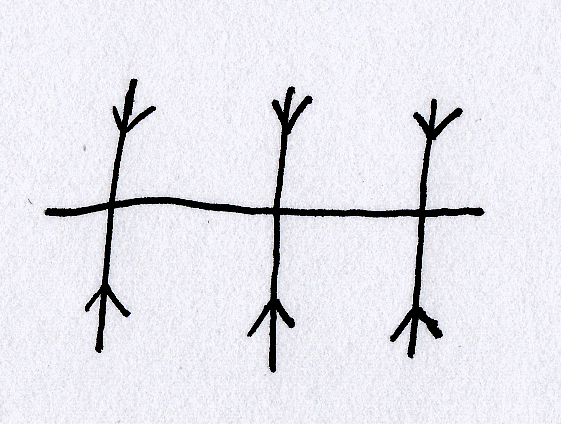
\includegraphics[scale = 0.15]{fig12.png}  & 
$ A = \left( \begin{array}{cc}
		0 & 0 \\
		 0 & \lambda \end{array} \right)   \quad(\lambda < 0) $ \\
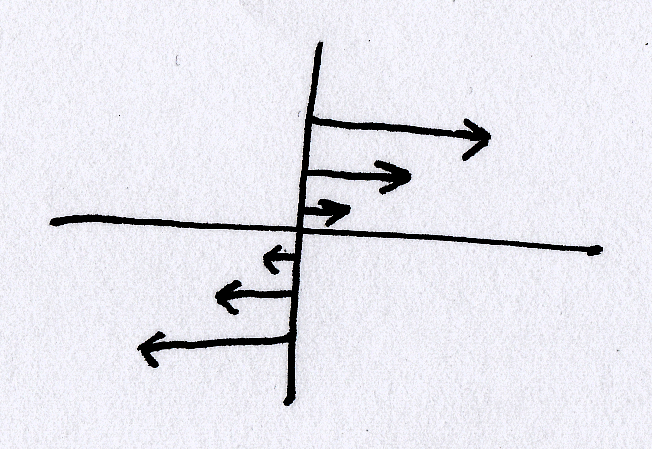
\includegraphics[scale = 0.15]{fig13.png}  & 
$ A = \left( \begin{array}{cc}
		0 & 1 \\
		 0 & 0 \end{array} \right)  $ 
\end{tabular}
\end{enumerate}
In summary 
\begin{figure}[H]
\centering
\includegraphics[width=14.4cm, height=10cm]{Diagram1.png}
\end{figure}
%
Notes:
\begin{enumerate}[(1)]
\item A Hamiltonian system is of the form
\[ \left( \begin{array}{c} \dot{x} \vspace{1mm}\\ \dot{y} \end{array} \right) =
\left( \begin{array}{r} \partial H / \partial y \vspace{1mm}\\ - \partial H / \partial x \end{array} \right) \]
for some $H(x,y)$. Fixed points are always saddles or centers because
\[ A = \left( \begin{array}{rr} H_{xy} & H_{yy} \\ -H_{xx} & -H_{xy} \end{array} \right) \implies T = 0 \]
Also $\dot{H} = \dot{\bm{x}}\cdot \nabla H = 0$ so the trajectories are
 (parts of) the contours of H.

\item The cannonical forms are obtained by using the eigenvectors $\bm{e}_i$ if
$\lambda _ i \in \mathbb{R}$ (possibly ``generalised'' for equal $\lambda$'s
and JNF, see Glendinning p 63) and $\mathrm{Re}(\bm{e}_1)$ and $\mathrm{Im}(\bm{e}_1)$ for 
$\lambda = \rho \pm i \omega$.

\item It is not necessary to change basis to classify the fixed point since
$T, \; D, \; \lambda$'s are invariant under $A \mapsto P^{-1}AP$, but knowing 
the eigenvectors may help sketch the phase diagram for the case of a saddle 
point.
\end{enumerate}
%
\textbf{Pertubation to A} (linear perturbations) 
\\
Cases (i)-(v) are robust - a small perturbation to A gives the same sort of 
eigenvalues and hence the same sort of fixed point.
\\
\\
Case (vi), if perturbed, may become a node or a focus, but these are 
topologically equivalent. The stability is not changed.
\\
\\
Cases (vii) and (viii) are fragile, - a small perturbation to (vii),
($\lambda = \pm i \omega$) may destroy the closed trajectories to give slow
spiralling inwards or outwards. A small perturbation to (viii) ($\lambda = 0$) 
may destroy the line of fixed points to give a slow drift towards/away from the
fixed point, and hence a saddle or node.
\\
\\
The fragility is because there are one or two eigenvalues on the border
Re$(\lambda) = 0$ between stability and instability.
\\
\\
\definition\ Hyperbolic fixed point
\\
\\
A fixed point $\bm{x}_0$ of the system $\dot{\bm{x}} = \bm{f}(\bm{x})$ is a
hyperbolic fixed point if none of the eigenvalues $\lambda$ of the Jacobian
$ \left. \frac{\partial f_i}{\partial x_j} \right| _{\bm{x} = \bm{0}} $ satisfy
Re$(\lambda) = 0$, and is non-hyperbolic otherwise.
\\
\\
In n-dimensions $(n \geq 0)$ we classify a hyperbolic fixed point as
\begin{enumerate}[(i)]
\item a sink if all eigenvalues have Re $(\lambda) < 0$.
\item a source if all eigenvalues have Re $(\lambda) > 0$.
\item a saddle point otherwise (some $>0$, some $<0$)
\end{enumerate}
In 2D
\begin{center}
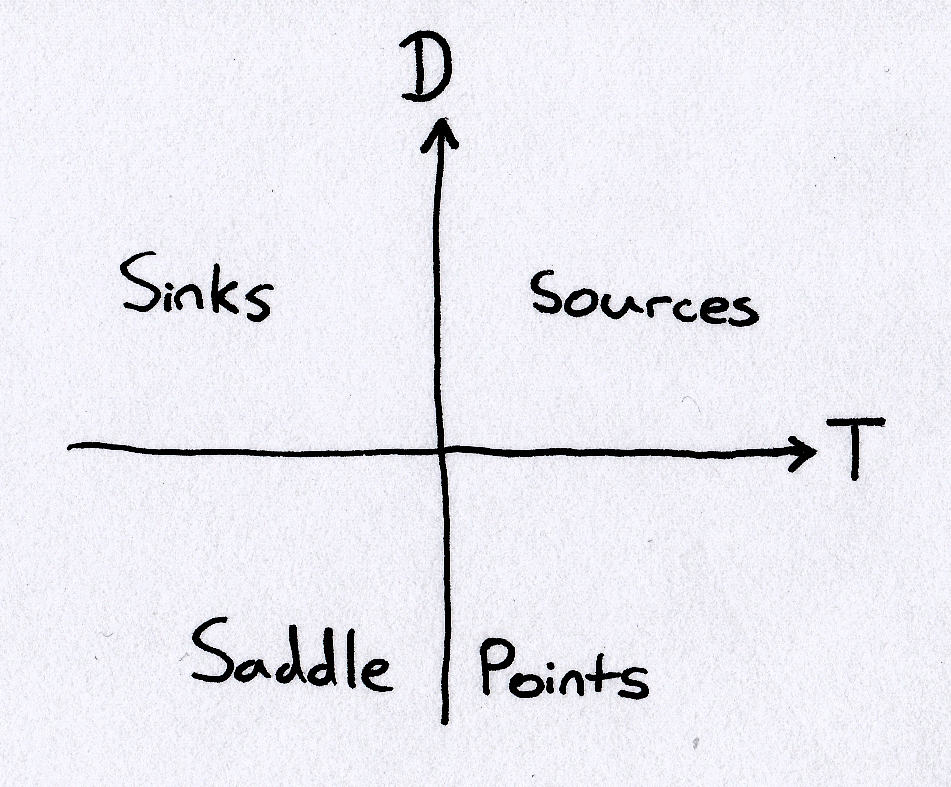
\includegraphics[scale = 0.15]{Diagram2.png}
\end{center}
% Diagram goes here!!
Non hyperbolic fixed points are important in bifurcation theory.
\\
\subsection{The effects of non-linear terms}
It is in fact true that the linearised system $\dot{\bm{y}} = A \bm{y}$
is essentially the same as the non linear system $\dot{\bm{x}} = \bm{f}(\bm{x})$
near a fixed point $\bm{x}_0$ provided
\begin{enumerate}[(i)]
\item The fixed point is hyperbolic
\item The non linear terms are $O( |\bm{x} - \bm{x}_0|^2)$
\end{enumerate}
(If (i) holds then the systems are topologically equivalent, if (ii) also holds,
then $\bm{h}(\bm{x})$ is a near identity map, so nodes are nodes and foci are
foci.)
\subsubsection{Stable and Unstable Manifold}
First, we formalise the idea of stable and unstable directions in the linearised
system.
\\
\\
\definition\ The stable, unstable and center invariant subspaces of the
linearisation of $\bm{f}$ at a fixed point are the local linear subspaces.
\\
\\
$E^s, \; E^u, \; E^c$ spanned by the eigenvectors of the Jacobian, whose 
eigenvalues have real parts $<0$, $ >0$,  $=0$ respectively. (Generalised
eigenvectors for JNF)
\\
\\
For some types of fixed point, these spaces may be empty, e.g. for a hyperbolic
fixed point, $E^c$ is empty by definition.
\\
\\
Then we extend th linear picture into the non-linear domain for a hyperbolic
fixed point.
\\
\\
\textbf{Stable Manifold Theorem}
\\
If $\bm{0}$ is a hyperbolic fixed point of the system $\dot{\bm{x}} = \bm{f}(\bm{x})$,
with linear stable and unstable invariant subspaces $E^s$ and $E^u$ then in a 
sufficiently small neighbourhood of the origin, there exist local stable and
unstable manifolds
\begin{align*}
W^s_{loc}(\bm{0}) &= \{ \bm{x} : \bp_t(\bm{x}) \to \bm{0} \mbox{ as } \
t \to \infty \} \\
W^u_{loc}(\bm{0}) &= \{ \bm{x} : \bp_t(\bm{x}) \to \bm{0} \mbox{ as } \
t \to -\infty \} 
\end{align*}
these have the same dimension as $E^s$ and $E^u$ and are tangent to them
at $\bm{0}$.
\\
\\
Notes:
\begin{enumerate}[(1)]
\item For a saddle point in $\mathbb{R}^2$, this guarantees the existence of
two specific trajectories (the separatrices) that approach and leave the saddle.
\item For a sink this guarantees that all trajectories in some neighbourhood of the
sink tend to it
\item The local stable (unstable) manifolds can be extended to global 
stable (unstable) invariant manifolds $W^s \; (W^u)$ by following the flow 
backwards (forwards).
\end{enumerate}
The proof of this is not in the course - See Glendinning.
\\
\\
It is easy to calculate approximations to $W^s$ and $W^u$ for a saddle point
in $\mathbb{R}^2$.
\\
\\
Wlog (Change of origin and basis) assume that the saddle is at $\bm{x}=\bm{0}$
and that $E^s$ is $x=0$ and $E^u$ is $y=0$.
\\
\\
\begin{tabular}{ m{4.5cm} m{9cm}  } 
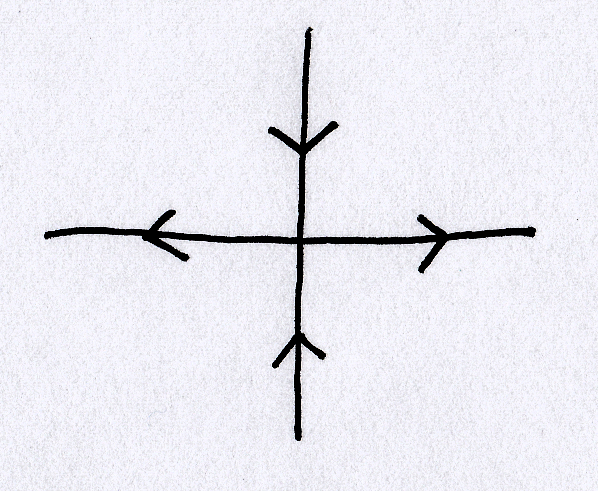
\includegraphics[scale = 0.15]{fig14.png}  & 

Then $W^s_{loc}$ becomes $x = S(y)$ with $S(0) =0, \; S'(0)=0$ 
$W^u_{loc}$ is $y = U(x)$ with $U(0) =0, \; U'(0)=0$.
\end{tabular}
\\
Since $W^s$ and $W^u$ are invariant,
\\
\[
 \left. \dot{x}\right|_{(S,y)} = \frac{dS}{dy} \left.\dot{y}\right|_{(S,y)} \qquad \qquad
 \left.\dot{y}\right|_{(x,U)} = \frac{dU}{dx} \left.\dot{y}\right|_{(x,U)}
\]
\\
\example\ 
\[ \left( \begin{array}{c} \dot{x} \\ \dot{y} \end{array} \right) = 
\left( \begin{array}{c} x - xy \\ -y+x^2 \end{array} \right) \qquad \qquad
A|_{\bm{x} = \bm{0}} = \left( \begin{array}{cr} 1 & 0 \\ 0 & -1 \end{array} \right) \]
Assume that
\[ y = U(x) = a_2 x^2 + a_3 x^3 + a_4 x^4 + \dots \]
substitute into 
\[ \dot{y} = U'\dot{x}  \implies -(a_2x^2+a_3x^3 + a_4x^4 + \dots) + x^2 
= (2a_2x + 3a_3x^2 + 4a_4x^3 + \dots)(x - a_2x^3 - \dots ) \]
Equate coefficients:
\begin{align*}
a_2 &= \frac{1}{3} \\
a_3 &= 0 \\
a_4 &= \frac{2}{45} \quad \mbox{etc.}
\end{align*}
Locally for $|\bm{x}| \ll 1$ \\
\begin{center}
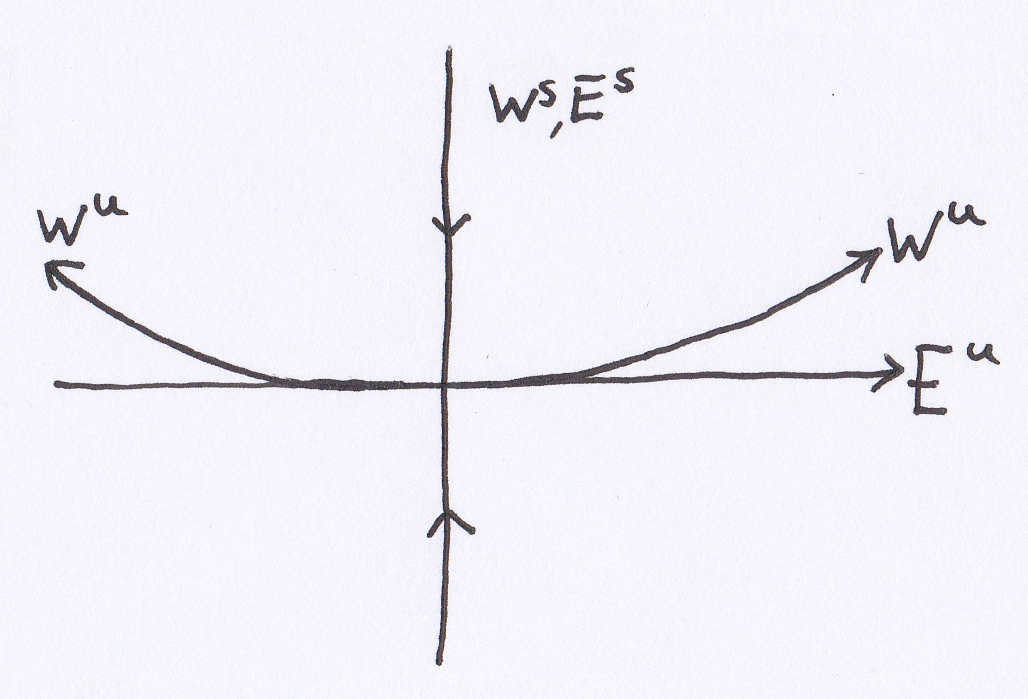
\includegraphics[scale = 0.15]{Diagram3.png}
\end{center}
In higher dimensions, would write $\bm{y} = \bm{U}(\bm{x})$ and solve
\[ \dot{y}_i = \frac{\partial U_i}{\partial x_i} \dot{x_j} \]
Where the $x_j$'s span $E^u$ and the $y_i$'s span $E^s$.
\subsubsection{Non-Linear terms in non-hyperbolic cases}
There are many possibilities depending on the non-linear terms.
\begin{enumerate}[(a)]
\item $\lambda = \pm i \omega$ Linear system is a centre. Are the trajectories
really closed?
\\
\\
\example\
\[ \left. \begin{array}{lr} 
				\dot{x} = & - y \pm x^3 \\
				\dot{y} = & x \pm y^3
\end{array} \right\} \implies \begin{array}{lr}
				\dot{r} = \pm \frac{x^4+y^4}{r} \\
			\dot{\theta} = 1 \pm \frac{xy^3-yx^3}{r^2} \end{array}\]
Now as $r \to 0$, $\dot{\theta} \to 1$. Thus the system is a stable focus if we choose '+'
and an unstable focus if we choose '$-$'.
\\
\\
\example\
\begin{alignat*}{4} 
& \dot{x} &&=  - && y - 2yx^2 =  &&\frac{\partial H}{\partial y} \\
& \dot{y} &&=    && x + 2xy^2 = -&&\frac{\partial H}{\partial x} 
\end{alignat*} 
for $H = - \frac{x^2+y^2}{2} - x^2y^2$. 
The trajectories are contours of H, which are closed near the maximum at 
$\bm{0}$. So the fixed point really is a non-linear centre with nested 
periodic orbits.
%
\item $\lambda_1 = 0$, $\lambda_2 \neq 0$. Which way does the system drift 
along $\bm{e}_1$?
\\
\\
\example\ \\ 
\begin{center}
\begin{tabular}{ m{3cm} m{3cm} m{3cm}  } 
$\begin{array}{lr}
 \dot{x} = & x^2 \\
 \dot{y} = & -y \end{array}$
& 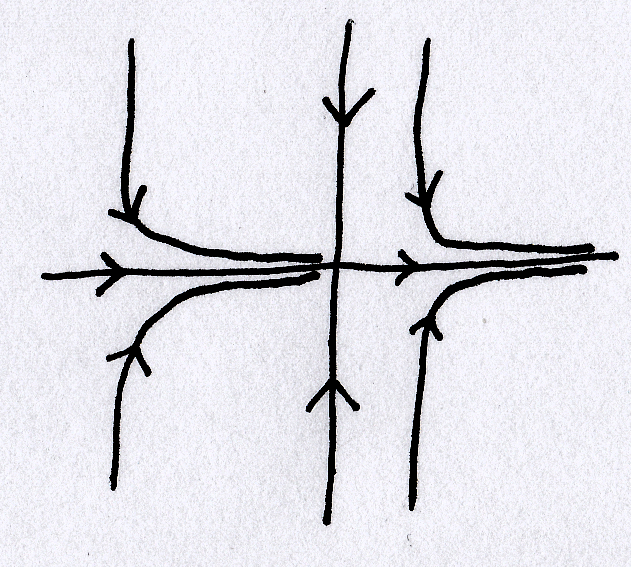
\includegraphics[scale=0.1]{fig15.png}
& Saddle-node \\ 
\\
\\
$\begin{array}{lr}
 \dot{x} = & x^3 \\
 \dot{y} = & -y \end{array}$
& 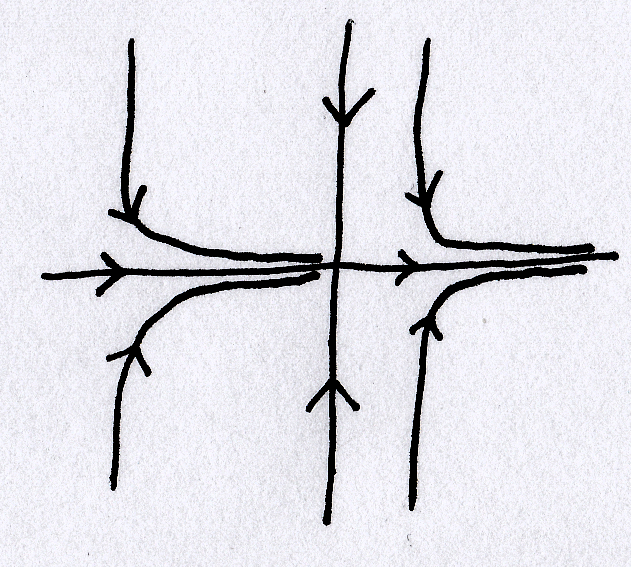
\includegraphics[scale=0.1]{fig15.png}
& Non-linear saddle
\end{tabular}
\end{center}
\item $\lambda_1 = \lambda_2 = 0$. Ad hoc methods needed.
\\
\\
In some cases, it is useful to switch to polars and consider the sign of
$\dot{r}$ and $\dot{\theta}$ as $r \to 0$.
\\
\\
\example\ $\dot{\theta} >0$ \\
\begin{center}
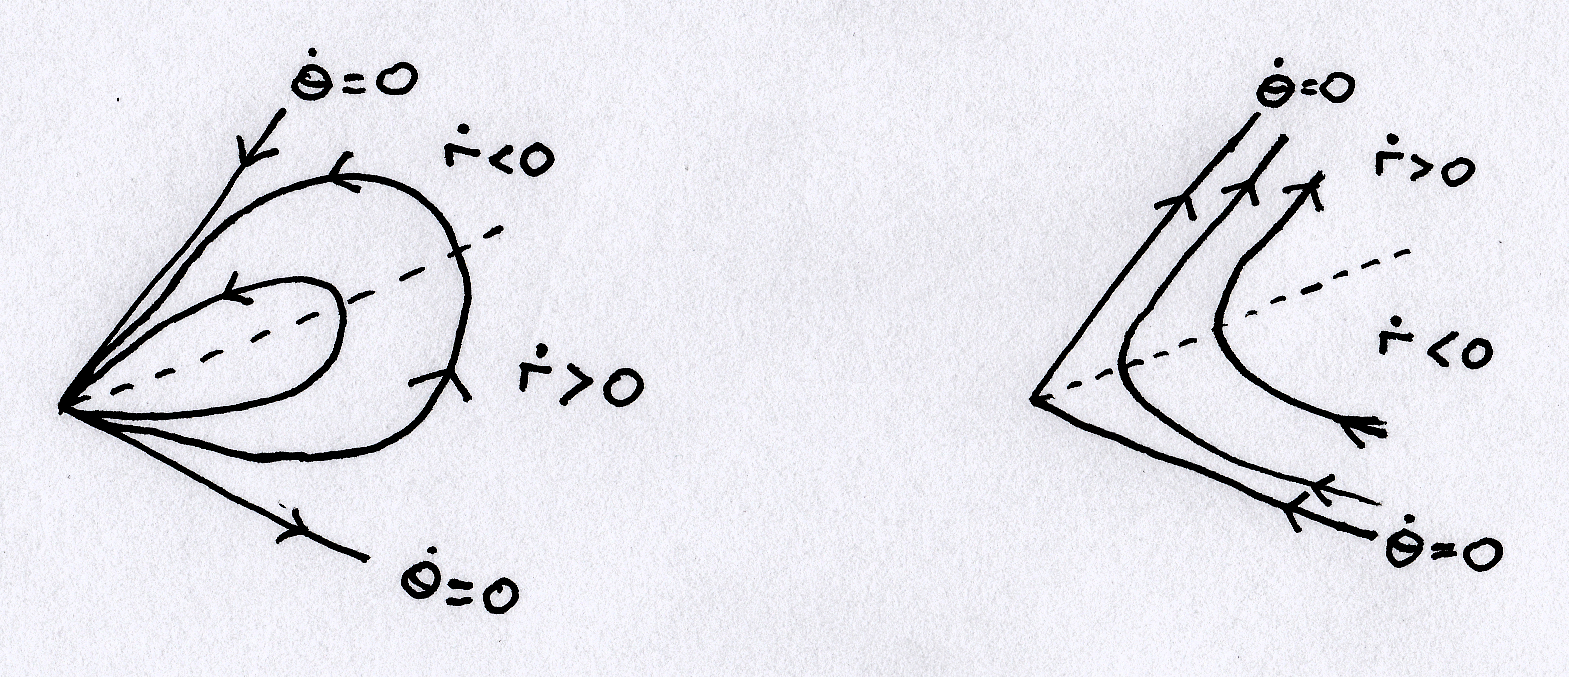
\includegraphics[scale = 0.15]{fig17.png} \\
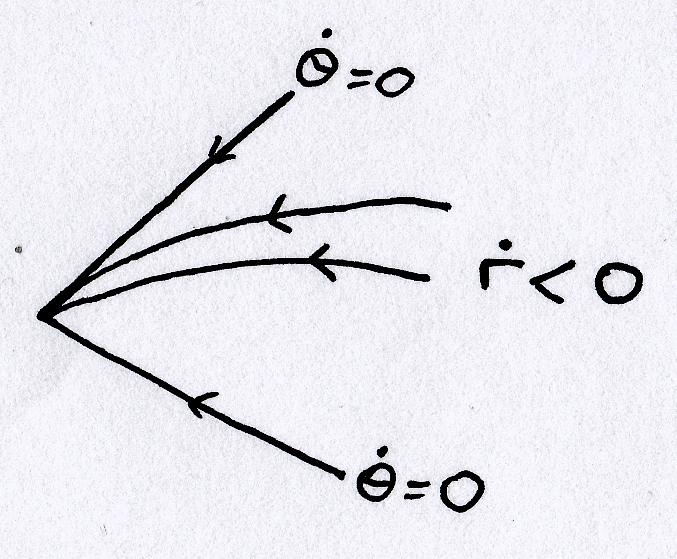
\includegraphics[scale = 0.16]{fig18.png}
\end{center}
In nastier cases, the curves $\dot{\theta} = 0$ can form a cusp.
\begin{center}
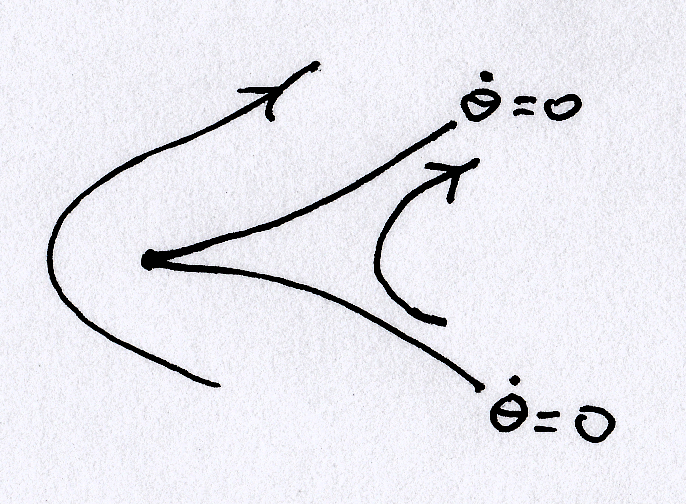
\includegraphics[scale = 0.16]{fig19.png}
\end{center}
\end{enumerate}
%
%
\subsection{Sketching phase planes/portraits}
%
\example\
\\
\begin{align*}
\dot{x} &= x(1-y) \\
\dot{y} &= -y + x^2
\end{align*}
This has fixed points at $(0,0)$ and at $(\pm1,1)$. 
\begin{center}
\begin{tabular}{ m{2cm} m{3cm} m{3cm} }
$(0,0)$ & $A = \left( \begin{array}{cr} 1 & 0 \\ 0 & -1 \end{array} \right)$ & saddle point \\ \\ \\
$(\pm 1,1)$ & $A = \left( \begin{array}{cr} 0 & \mp 1 \\ \pm 2 & -1 \end{array} \right)$ & stable foci
\end{tabular}
\end{center}
It is clear why $(0,0)$ is a saddle point. For $(\pm1,1)$ observe that 
$T=-1$, $D=2$, $T^2 < 4D$, and therefore $(\pm 1, 1)$ are stable foci. Before
sketching, observe that.
\begin{itemize}
\item $x = 0$ is a trajectory.
\item $\dot{x}=0$ on $y=1$
\item $\dot{y} = 0$ on $y=x^2$
\item $\dot{y} \,\, ^{<}_{>} \,\, 0$ if $y \,\,^{<}_{>} \,\, x^2$
\item Symmetry in y axis; under $x \mapsto -x$, $\dot{x} \mapsto -\dot{x}$, and $\dot{y} \mapsto \dot{y}$
\item Know that the unstable manifold is given by $y \approx \frac{1}{3} x^2 + \frac{2}{45} x^4$
near $x=0$ (See earlier example)
\end{itemize}
Put all of this together to sketch the following:
\begin{figure}[H]
\centering
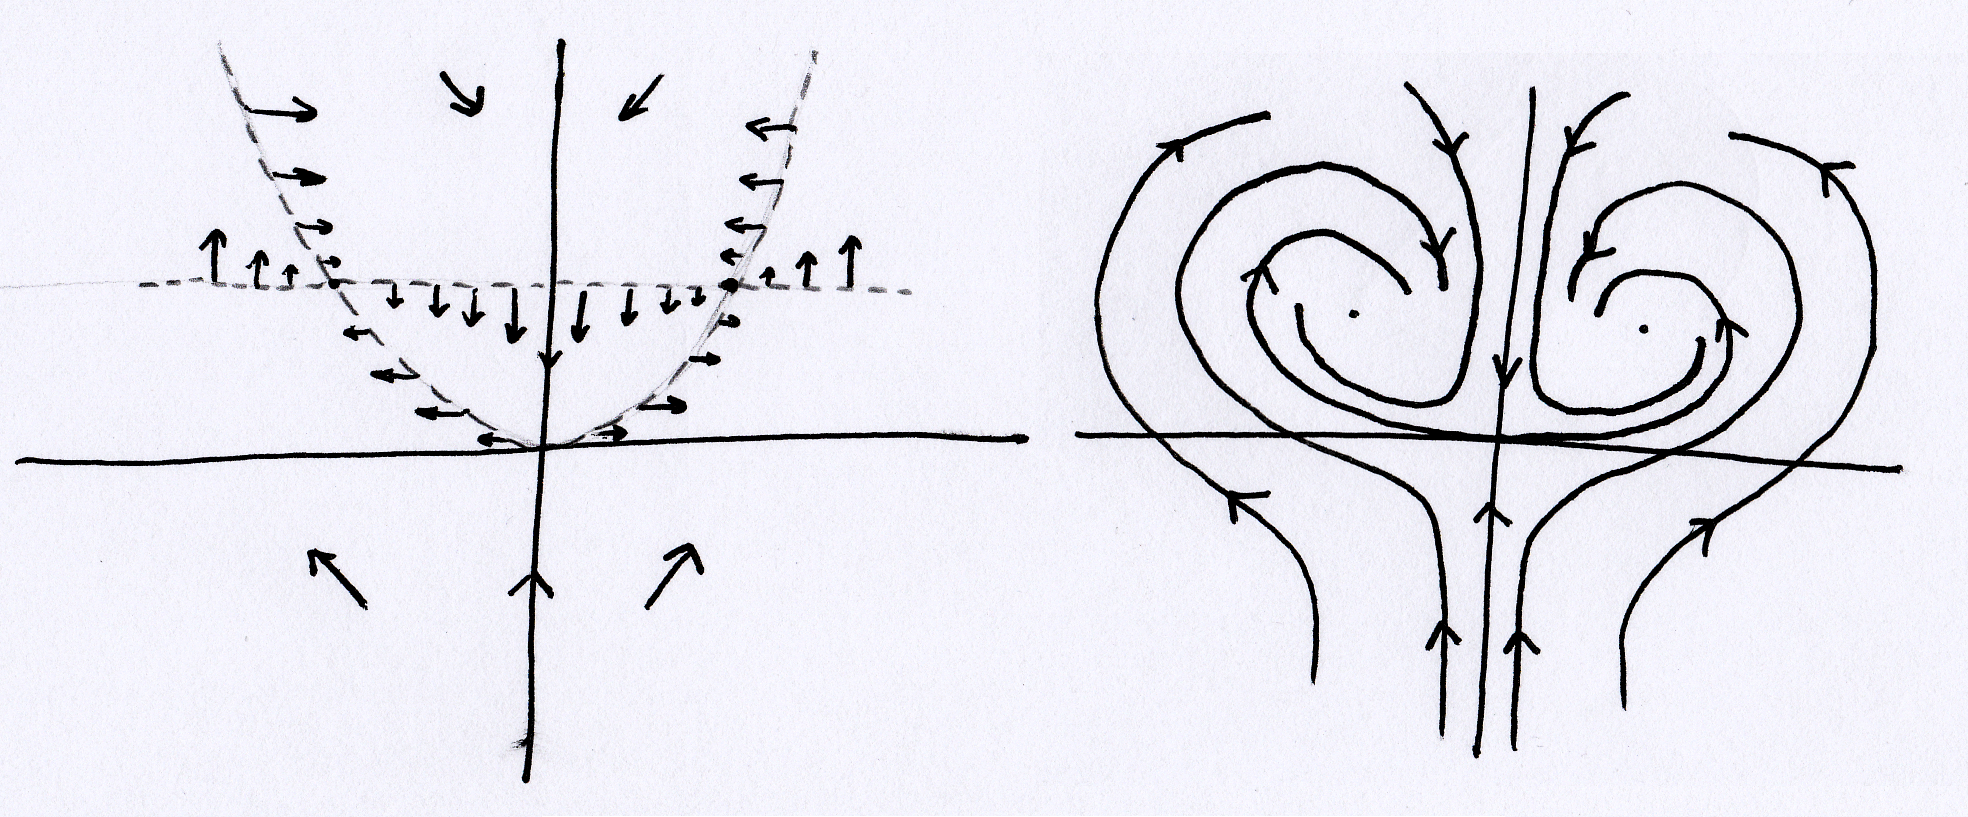
\includegraphics[scale=0.2]{fig20.png}
\end{figure}
\noindent In general, here are some steps to follow when sketching a phase plane.
\begin{enumerate}[1.]
\item Find the fixed points.
\item \begin{enumerate}[(a)] \item Calculate the Jacobian to find the kind of eigenvalues and classify
				the fixed points.
				\item If any are non-hyperbolic, consider non-linear terms, possible
				Hamiltonian structure, signs of $\dot{x}$, $\dot{y}$, $\dot{r}$ or 
				$\dot{\theta}$ as $|\bm{x} - \bm{x}_0| \to 0$.
      \end{enumerate}
\item Calculate the eigenvectors for saddles.
\item Consider the sign of $\dot{x}$ and $\dot{y}$ - the curves where these are
zero are called nullclines.
\item Construct the global picture by joining up the local behaviour near fixed
points. (especially the separatrices of saddles) using the arrows from $\dot{x}$
and $\dot{y}$.
\item At some stage, decide whether there are periodic orbits.
\end{enumerate}
%
%
%
For an additional example, see handout 2.4, ``Example of Phase-Plane sketching.''
\section{Stability}
\subsection{Definitions}
It is clear what it means for a hyperbolic node or focus to be stable, but we
ned to be more careful with the stability of other kinds of fixed points or 
invariand sets, because there are at least two notions of stability.
\\
\\
\definition\ Lyapunov stability
\\
A fixed point $\bm{x}_0$ of a flow $\bp_t$ is Lyapunov stable if
$\forall \epsilon > 0, \; \exists \delta > 0$ s.t. $|\bm{x}-\bm{x}_0| < \delta$
$\implies |\bp_t(\bm{x}) - \bm{x}_0| < \epsilon$ $\forall t>0$.
A motto is ``Start near, stay near'' stability.
\\
\\
\definition\ Quasi-asymptotic stability (QAS)
\\
A fixed point $\bm{x}_0$ of a flow $\bp_t$ is quasi-asymptotically 
stable if $\exists \delta > 0$ s.t. $|\bm{x}-\bm{x}_0| < \delta$ $\implies
\bp_t(\bm{x}) \to \bm{x}_0$ as $t \to \infty$.
\\
\\
These are not the same!
\\
\\
\example\
\\
\begin{tabular}{m{3cm} m{4cm} m{9cm}  } 
$\begin{array}{lr} 
\dot{r} = & 0 \\
\dot{\theta} = & 1
\end{array}$ &
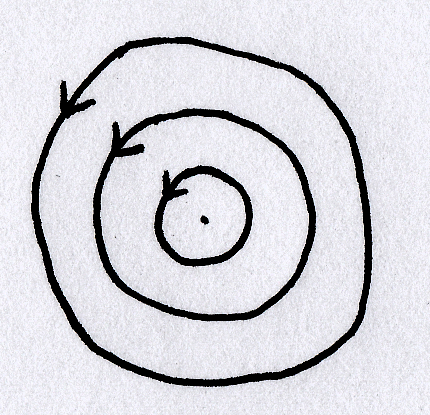
\includegraphics[scale = 0.15]{fig11.png}  & 
Lyapunov stable, but not asyptotically stable.
\\
\\
$\begin{array}{lr} 
\dot{r} = & r(1-r^2) \\
\dot{\theta} = & \sin^2(\theta/2)
\end{array}$ &
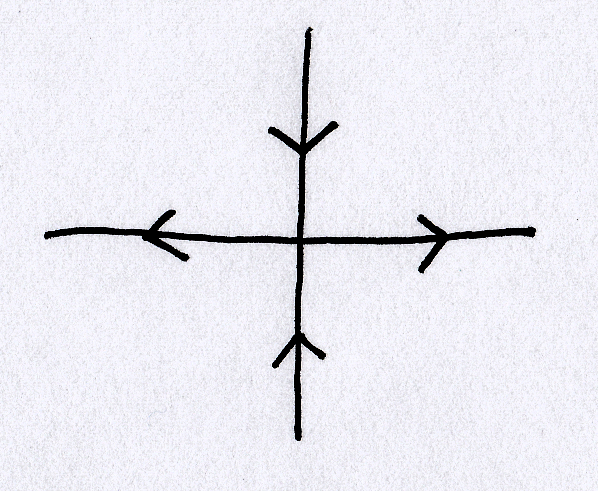
\includegraphics[scale = 0.15]{fig14.png}  & 
The point $r=1$, $\theta = 0$ is QAS but not Lyapunov stable
\end{tabular}
\\
\\
\definition\ Asymptotic stability (AS)
\\
A fixed point $\bm{x}_0$ is asymptotically stable if it is both Lyapunov stable
and quasi-asymptotically stable.
\\
\\
\example\ A sink (Re $\lambda_i <0 \; \forall \, i$) is asymptotically
stable. (Choose $\delta$ sufficiently small that the linear terms dominate)
A saddle or source is obviously not Lyapunov stable, hence not AS.
\\
\\
For other kinds of invariant sets $\Lambda$ e.g. limit cycles, define
\[ N_{\delta}(\Lambda) = \{ \bm{x} : \exists \bm{y} \in \Lambda \mbox{ with } \
|\bm{x} - \bm{y}| < \delta \} \]
and say 
\[ \bp_t(\bm{x}) \to \Lambda\]
if
\[\min_{\bm{y} \in \Lambda} \
\{ | \bp_t(\bm{x}) - \bm{y}| \} \to 0 \quad \mbox{ as } \quad t \to \infty \]
\\
Then say $\Lambda$ is Lyapunov stable if $\forall \epsilon > 0$ $\exists \delta>0$ s.t.
$\bm{x} \in N_{\delta}(\Lambda) \implies \bp_t(\bm{x}) \in N_{\epsilon}(\Lambda)$
$\forall t >0$.
\\
\\
Say $\Lambda$ is QAS if $\exists \delta >0$ s.t. $\bm{x} \in N_{\delta}(\Lambda) \implies \
\bp_t(\bm{x}) \to \Lambda$ as $t \to \infty$.
\\
\\
Say $\Lambda$ is AS if it is both LS and QAS.
\\
\subsection{Lyapunov functions}
These allow us to say more about the stability of a fixed point which wlog
we take to be $\bm{x}=0$.
\\
\\
\definition\ Lyapunov function
\\
A continously differentiable function $V : \mathbb{R}^n \to \mathbb{R}$ is a Lyapunov
function for $\xeq{x}$ in a domain $\mathcal{D} \subset \mathbb{R}^n$ if
%
\begin{enumerate}[(i)]
\item $V(\bm{0}) = 0$ and $V(\bm{x}) > 0$ for 
      $\bm{x} \in \mathcal{D} \backslash \{\bm{0}\}$.
     ``\emph{Positive semi-definite}''.

\item $\dot{V}(\bm{x}) \equiv \bm{f}\cdot \nabla V \leq 0$
      $\forall \bm{x} \in \mathcal{D}$. ``\emph{Non-increasing}''.

\end{enumerate}
%
Note that (ii) means trajectories head ``downhill'' (or at least not uphill)
and (i) means that $\bm{0}$ is the lowest point. These properties allow us to
prove:
\\
\\
\theorem\ Lyapunov's First Theorem
\\
If a Lyapunov function exists, then $\bm{0}$ is Lyapunov stable.
\begin{proof}
Wlog we can assume $\epsilon$ is sufficiently small that 
$\{ | \bm{x} | < \epsilon \} \subset\mathcal{D}$. Let
\[ m = \inf \{ V(\bm{x}) : | \bm{x} | = \epsilon \} \]
$m$ is attained, and $m>0$ since $\{ |\bm{x}| = \epsilon \}$ is compact.
Define
\[ C_{m, \epsilon}  = \{ \bx : V(\bx)<m \mbox{ and } |\bx| < \epsilon \} \]
Then $\bx \in C_{m,\epsilon} \implies \bp_t(\bx) \in C_{m,\epsilon}$ 
$\forall \, t>0$ since V is non-increasing and $V \geq m$ on the
boundary of $C_{m,\epsilon}$. 
\\
\\
Finally, choose $\delta >0$ such that 
$\{ |\bx| < \delta \} \subset C_{m,\epsilon}$. Then
\\
\[|\bx|< \delta \implies |\bp_t(\bx)|<\epsilon \;\; \forall \, t>0 \]
% Include diagram here
\end{proof}
%
%
\noindent
A trajectory can head downhill and still not end up at $\bm{0}$.
However, there is an important constraint.
\\
\\
\theorem\ La Sale's Invariance Principle
\\
If V is a Lyapunov function on a bounded domain $\domain$ and
$\cO^+(\bx) \subset \domain$, then $\bp_t(\bx) \to$ an invariant subset of
$\{ \bx : \dot{V}(\bx) = 0 \} $.
%
\begin{proof} ~
\\
$\cO^+(\bx) \subset \domain$ so $V(\bp_t(\bx))$ is monotonically decreasing
and bounded below by $0 \implies V(\bp_t(\bx)) \to \alpha$ for some 
$\alpha \geq 0$ as $t \to \infty$.
\\
\\
$\domain$ is bounded $\implies \omega(\bx)$ is non empty.
\\
\\
Let $\bm{y} \in \omega(\bx)$ then 
$\exists \, \{t_n\}$ s.t. $\bp_{t_n}(\bx) \to \bm{y} \implies V(\bm{y}) = \alpha$ 
by continuity of V.
\\
\\
Therefore $V(\bp_t(\bm{y})) = \alpha$ since $\bp_t(\bm{y}) \in \omega(\bx)$.
\\
\\
Now $V(\bp_t(\bm{y})) = \alpha \;\; \forall \, t \implies \dot{V}(\bm{y}) = 0$.
\\
\\
This holds for any $\bm{y} \in \omega(\bx)$ and thus
\[ \omega(\bx) \subset \{ \dot{V} = 0 \} \]
We know $\omega$ is invariant, and thus we are done.
\end{proof}
\noindent \textbf{Corollary:} If V is a Lyapunov function on a domain $\domain$ 
containing $\bm{0}$, and the only invariant subset of 
$\{ \bx:\dot{V}(\bx) = 0\} \cap \domain$ is $\{ \bm{0} \}$, then $\bx = \bm{0}$
is asymptotically stable.
%
\begin{proof} ~
\\
Choose $k$ such that 
\[ C_k \equiv \{ \bx : V(\bx) <k \} \subset \domain \]
and choose $\delta$ such that $ \{ \bx :| \bx | < \delta \} \subset C_k$.
\\
Then $|\bx| < \delta \implies V(\bx) <k \implies V(\bp_t(\bx)) < k \implies \
\bp_t(\bx) \subset \domain$
\end{proof}
\noindent \\ \\
\example\ Let
\[\dot{\bx} = A \bx + o(|\bx|)\]
and let $\lambda_i$ be the distinct eigenvalues of A with corresponding 
eigenvectors $\bm{e}_i$.
\\ 
Suppose that Re$(\lambda_i) <0$,and let $v_i$ be any positive real
constants. Then, writing 
\[ \bx = \sum_{i=1}^{n} a_i \bm{e}_i, \qquad V(\bx) = \sum_{i=1}^{n} v_i |a_i|^2\]
have that $V \geq 0$ ($=0$ only at
$\bm{0}$) and $\dot{V}$ in a sufficiently small neighbourhood of $\bm{0}$.
(See example sheet) Therefore have that $\bx = \bm{0}$ is asymptotically
stable.
\\
\\
The main use of Lyapunov functions, however, is to find information about the
domain of stability.
\\
\\
\definition\ Domain of stability
\\
The domain of stability (basin of attraction) of an asymptotically stable
invariant set $\Lambda$ is 
\[ \{ \bx : \bp_t(\bx) \to \Lambda \mbox{ as } t \to \infty \} \]
i.e. $\bx$ such that 
\[ \inf_{\bm{y} \in \Lambda} \{| \bp_t(\bx) - \bm{y} | \} \to 0 \quad \mbox{as } t \to \infty\]
\\
If the domain of stability in $\mathbb{R}^n$ then $\Lambda$ is globally stable.
\\
\\
\example\ We can show that the non-hyperbolic fixed point of the system
\begin{align*}
 \dot{x} =& y-xy^2 \\
 \dot{y} =& x^3
\end{align*}
is asymptotically stable.
\\
\\
Without the $-xy^2$ term, the system would be Hamiltonian with 
$H = \frac{1}{2}y^2+\frac{1}{4}x^4$ and $\dot{H}=0$.
\\
With the $-xy^2$ term, $\dot{H} = -x^4 y^2 \leq 0$.
\\
Therefore $H$ is a Lyapunov function and so $\bp_t(\bx) \to$ an invariant
subset of $\{\dot{H}=0\} = \{ x = 0 \mbox{ or } y = 0 \}$.
\\
But the only invariant subset of $\{ \dot{H} = 0 \}$ is $\bx = \bm{0}$.
Hence by the corollary, $\bx = \bm{0}$.
\\
\\
\example\
\[ \left. \begin{array}{cl} \dot{x} = & y + \mu ( \frac{1}{3} x^3 - x) \\
			    \dot{y} = & -x \end{array}
\right\} \mbox{ equivalent to } \ddot{x} + \mu (1 - x^2) \dot{x} + x = 0 \]
The ``Time-reversed van der Pol oscillator''. Observe that $\bx = \bm{0}$ 
is a sink for $\mu >0$.
\\
\\
Guess $V = x^2 + y^2$ (e.g. from case $\mu = 0$). This implies that
$\dot{V} = 2 \mu x^2 ( \frac{x^2}{3} -1)$ so $\dot{V} \leq 0$ in $x^2 <3$.
%Include a figure here
\\
Let $C_3 = \{ V < 3 \}$ so $\bx \in C_3 \implies \bp_t(\bx) \in C_3$.
\\
\\
La Salle's invariance principle $\implies \bx \in C_3$ then $\bp_t(\bx)$ tends
to an invariant subset of $\{ \dot{V}=0 \}$. But the only invariant subset of
$\{ x = 0 \}$ is $\{ x = y =0\} \implies \bm{0}$ is AS and the domain of
stability \underline{includes} $C_3$. 
\\
\\
\textbf{General method}
\begin{enumerate}[(1)]
\item Find a domain $\domain$ and function V such that
	\begin{enumerate}[(i)]
	\item $V \geq 0$ on $\domain$ and $V=0$ iff $\bx = \bm{0}$
		(easy)
	\item $\dot{V} \leq 0$ on $\domain$ (harder, often restricts the 
		size of $\domain$ )
	\end{enumerate}
\item Choose $k$ such that $C_k = \{V<k\} \subset \domain$.
\item If necessary, adjust $k$ (or V), so that the only invariant subset of
      $\{ \dot{V} = 0 \} \cap C_k$ is $\bx = \bm{0}$. Then La Salle implies
      that the origin is AS stable \underline{and} the domain of stability
      includes $C_k$.
\item Try different $V$ to maximise $C_k$ or take a union of them.
\end{enumerate}
\example\
\[ \left. \begin{array}{cl} \dot{x}  &= -x +xy^2 \\
			    \dot{y}  &= -y +yx^2 \end{array}
\right\} \mbox{ Try } V = x^2 +by^2 \]
\[ \implies \dot{V} = -2(x^2+b^2y^2) + 2(1+b^2)x^2y^2\]
Clearly $\dot{V} \leq 0$ sufficiently close to $\bm{0}$.
\\
Let $(x,by) = \sqrt{V}(\cos \phi, \sin \phi )$
\\
\[ \implies \dot{V} = -2V + 2V^2 \left( \frac{1+b^2}{b^2} \right) \
\underbrace{\cos ^2 \phi \sin ^2 \phi}_{\leq \, 1/4} \]
\[ \implies \dot{V} \leq 0 \mbox{ in } 0 \leq V \leq \frac{4b^2}{1+b^2} \]
The domain of stability includes the union over $b$ of these regions.
% Small picture here!
\\
\\
For another example see handout 3.2, ``Examples of Domains of Stability''.
\subsection{Bounding Functions}
The idea of a function decreasing along trajectories.
\\
If V is a function with bounded contours and $\dot{V} < \delta <0$ in the
region $V(\bx) >M$, then all trajectories eventually enter and remain in 
the set $\{ V(\bx) < M \}$. Such a V is called a bounding function.
% Another figure
\\
%%%%%%%%%%%%%%%%%%%%%%%%%55
\section{Existence and Stability of Periodic orbits in $\mathbb{R}^n$}
There is a toolkit of standard techniques, particular to $\mathbb{R}^2$, 
to prove that there either is or isn't one or more periodic orbits.
\\
\subsection{Poincar\'{e} index test}
Consider 
\[ \left( \begin{array}{c} \dot{x} \\ \dot{y} \end{array} \right) = \
 \left( \begin{array}{c} f_1 \\ f_2 \end{array} \right) \]
Except at a fixed point $(\bm{f} = \bm{0})$, the trajectory through a point
$\bx$ makes a well defined angle $\psi(\bx)$ with the $x$-axis.
% A little picture goes here.
\\
\\
\definition\ Poincar\'e index of a curve
\\
If $\Gamma$ is a simple closed curve, not necessarily a trajectory, that
doesn't pass through any fixed points,  then moving around $\Gamma$ once
anticlockwise, $\psi = \tan^{-1} \frac{f_1}{f_2}$ changes continously and
returns to its original value plus an integer multiple of $2\pi$. This multiple
is the Poincar\'e index $I(\Gamma)$ of $\Gamma$.
\\
\\
Properties:
\begin{enumerate}[1.]
\item %
\[ 2\pi I(\Gamma) = \oint_{\Gamma} d\psi = \oint_{\Gamma} d\left( \tan^{-1} \
\frac{f_1}{f_2} \right) = \oint_{\Gamma} \frac{ f_1 df_2 - f_2 df_1}{f_1^2 + f_2^2} \]
\item $I(\Gamma)$ is unchanged by deformations of $\Gamma$ that do not cross 
a fixed point. 
\\
(Proof: $I(\Gamma)$ is integrable and a continous function of $\bm{f}$
(from 1) provided $\bm{f} \neq \bm{0}$.
\item If $\Gamma$ encloses no fixed points, then $I(\Gamma) =0$.
\item The Poincar\'e index is additive,
% Insert a figre here
$I(\Gamma_1) = I(\Gamma_2) + I(\Gamma_3)$
\item If $\Gamma$ is a closed trajectory, i.e. a periodic orbit, then 
$I(\Gamma)=1$. % Insert another picture here
\item If time is reversed $(\bm{f} \to -\bm{f})$ then $I(\Gamma)$ is unaffected
(from 1).
\\
\\
\definition\ Poincar\'e index of a fixed point
\\
The Poincar\'e index of an isolated fixed point is the Poincar\'e index of any
simple closed curve enclosing this fixed point and no others. (Well defined by 
2.)
\\
\item $I(\Gamma)$ is the sum of the Poincar\'e indices of the fixed points it 
encloses.
\item The Poincar\'e index of a node, focus, or center is $+1$.
% A figure goes here
\item The Poincar\'e index of a saddle is $-1$.
% Another figure goes here
\end{enumerate}
Non-hyperbolic fixed points other than centers need to be done on a case
by case basis.
\\
\\
\example\ $\dot{x} = x^2, \quad \dot{y} = -y$
\\ 
Index = 0
% Another figure goes here.
\\
\\
\textbf{Important Corollaries} \\
If there are any periodic orbits, then each must contain at least one fixed point.
The fixed point(s) enclosed by a periodic orbit must have indicies summing to $+1$.
\\
\\
If the above is not possible then there are no periodic orbits. This is the 
Poincar\'e index test. (a negative test)
\\
\\
\example\
\begin{align*}
\dot{r} &= r(3 - r -s) \\
\dot{s} &= s(2 - r -s)
\end{align*}
Any periodic orbit canot cross the trajectories $r=0$ and $s=0$. Therefore
it cannot enclose any of the nodes. A periodic orbit cannot enclose only the
saddle (index $-1$), hence there are no periodic orbits.
\\
\subsection{Dulac's Criterion}
Another negative test.
\\
\\
\theorem\ Dulac's criterion
\\
If there is a continously differentiable funciton $\phi(x,y)$ such that
$\nabla \cdot ( \phi \bm{f}) \neq 0$ in a simply connected domain 
$\domain \subset \mathbb{R}^2$ then there are no periodic orbits lying
entirely within $\domain$.
\begin{proof} ~
\\
Assume, wlog, $\nabla \cdot ( \phi \bm{f} ) > 0$, suppose that $\Gamma$ is
a periodic orbit lying entirely in $\domain$, and enclosing an area A with
outward normal $\bm{n}$.
% A diagram here...
\[ \int_{\Gamma} \phi \bm{f} \cdot \bm{n} \, ds = 0 = \int_{A} \nabla \
\cdot ( \phi \bm{f} ) dA \; >0 \]
which is a contradiction.
\end{proof}
%
\noindent Often we just take $\phi = 1$, this is known as the divergence test.
\\
\\
\corollary\ If $\nabla \cdot ( \phi \bm{f}) \neq 0 $ in a doubly connected
domain $\domain$, then there is at most one periodic orbit lying entirely in
$\domain$.
\begin{proof}
Apply the divergence theorem to the area between two hypothetical periodic 
orbits in $\domain$.
\end{proof}
\noindent
\example\   The Lotka-Voltera equations
\begin{align*}
\dot{r} &= r(a - br -cs) \\
\dot{s} &= s(d - er -fs)
\end{align*}
Choose $\phi = \frac{1}{rs}$. Then $\nabla \cdot ( \phi \bm{f}) = \
-\frac{b}{s} - \frac{f}{r} <0$ in $r,s \, >0$, for $b,f \, >0$.
Therefore there can be no periodic orbits entirely in $r,s \, > 0$.
\\
\\
\example\ Damped pendulum with torque
\\
\begin{align*}
\dot{\theta} &= p \\
\dot{p}      &= F - kp - \sin \theta
\end{align*}
The argument is slightly complicated by the phase space having the topology 
of a cylinder.
\\
% Figure of a cylinder
Can work on the cylinder and use $\frac{\partial \dot{\theta}}{\partial \theta} +\
\frac{\partial \dot{p}}{\partial p} = -k <0$ to deduce that there is at most one
periodic orbit, which must encircle the cylinder.
\\
\\
Alternatively can let $r = e^p$ to map onto plane polars, and use $\phi = 1/r^2$,
\[ \nabla \cdot (\phi \bm{f}) = \nabla \cdot ( \phi( \dot{r} \bm{e}_r + r \
\dot{\theta} \bm{e}_{\theta})) = -\frac{k}{r^2} < 0\]
\\
\\
\subsection{Poincar\'e-Bendixson Theorem}
A positive test!
\\
\\
\theorem\ Poincar\'e-Bendixson
\\
If the forward orbit $\cO^+(\bx)$ of a point $\bx$ remains in a compact 
(closed and bounded) set $K \subset \mathbb{R}^2$, and $K$ contains no 
fixed points, then $\omega(\bx)$ is a periodic orbit.
\\
\\
Note:
\begin{enumerate}[1.]
\item From 3.1, $K$ must be multiply connected with a fixed point in one
	of the holes.
\item Idea: The trajectory must go somewhere, and the conditions of the 
	theorem mean it can't go to $\infty$ or a fixed point.
\end{enumerate}
% A figure goes here
The full (sketch) proof is in handout 4.4.\\
\example\
\begin{align*}
\dot{x} &= x - y - 2x(x^2+y^2) \\
\dot{y} &= x+y -y(x^2+y^2)
\end{align*}
The linear terms $\implies \bm{0}$ is an unstable foci. The cubic terms
look inward from $-\infty$.
\\
Try for an annulus in polar coordinates
\[ \dot{r} = \frac{1}{r}(x^2+y^2)(1-2x^2-y^2) = r(1-r^2(1+\cos^2 \theta)) \]
minimising/maximising over $\theta$ gives
\[ r(1-2r^2) \leq \dot{r} \leq r(1-r^2) \]
and therefore
\begin{align*}
\dot{r}>0 &\mbox{ in } r < \frac{1}{\sqrt{2}} \\
\dot{r}<0 &\mbox{ in } r > 1
\end{align*}
So trajectories entering the annulus $C = \{ \frac{1}{\sqrt{2}} \leq r \leq 1 \}$
remain there.
\\
No other fixed points?
\[\dot{\theta} = \frac{x \dot{y} - y \dot{x}}{r^2} = 1 + \frac{1}{2}r^2 \sin \
2\theta \implies \dot{\theta} > 0 \mbox{ in } r < \sqrt{2} \]
$C$ contains no fixed points. By Poincar\'e-Bendixson theorem, $C$ contains a
periodic orbit.
\\
\\
( $\nabla \cdot \bm{f} = 2 - 5r^2 -2x^2 <0$ in $C$, therefore there is
only one periodic orbit)
\\
\\
\example\ Forced damped pendulum again
\begin{align*}
\dot{\theta} &= p \\
\dot{p}      &= F - kp - \sin \theta
\end{align*}
From bounding functions in \S 3.3, we know that all trajectories enter
and remain in the compact set
\footnote{I actually have no idea what V is! my notes don't contain any 
reference, and apparently I didn't notice at the time...}
\[ V \leq \frac{1}{2} \left(\frac{F}{k} \right)^2 +2\]
If $F>1$ then there are no fixed points $\implies$ there is a periodic
orbit by Poincar\'e-Bendixson. (and only one by corollory to Dulac's
criterion)
\\
\subsection{Nearly Hamiltonian Flows}
This can be a negative or positive test.
\\
\\
Consider a system 
\begin{align*}
\dot{x} &= f_1(x,y) + \epsilon g_1(x,y) \\
\dot{y} &= f_2(x,y) + \epsilon g_2(x,y) 
\end{align*}
Where
\[ f_1 = \frac{\partial H}{\partial y}, \qquad f_2 = -\frac{\partial H}{\partial x}\]
If $\epsilon =0$ then $\dot{H} = 0$ and closed contours of $H$ are periodic 
orbits. If $\epsilon \neq 0$ then 
\[\dot{H} = \frac{\partial H}{\partial x} \dot{x} + \frac{\partial H}{\partial y}\
\dot{y} = \epsilon \dot{x} g_2 - \epsilon g_1 \dot{y} = \epsilon(g_2f_1-g_1f_2) \]
For a periodic orbit $\Gamma$, we must have
\[ \oint_{\Gamma} dH = 0 \implies \oint_{\Gamma} \epsilon (g_2f_1 - g_1f_2) dt = 0\]
Hence there are no periodic orbits that lie entirely in a region where 
$g_2f_1 - g_1f_2 > 0$ (or $<0$).
\\
\\
If $0< \epsilon \ll 1$ then $\dot{H} = O(\epsilon)$, therefore the trajectories 
of the peturbed system are very similar to the contours of $H$.
So changes in $H$ can be approximated by integrating along the trajectories
$H=H_0$ of the unpeturbed Hamiltonian system.
\[ \Delta H(H_0) = \epsilon \oint_{H=H_0} (g_2 f_1 - g_1 f_2)dt + O(\epsilon ^2) \
= \epsilon \oint_{H=H_0} g_2dx - g_1dy + O(\epsilon^2) \]
Where the $O(\epsilon^2)$ terms arise as the trajectory is not exactly $H=H_0$.
\\
\\
Fixed points $\Delta H = 0$ of the energy return map 
$H_{n+1} = H_n + \Delta H(H_n)$ correspond to periodic orbits. Finding 
approximations to them by neglecting the $O(\epsilon^2)$ terms is called the 
energy balance equation.
\\
\\
Note that the $O(\epsilon^2)$ can make a double root of $\Delta H =0$ 
disappear, but not a single root.
\\
\\
\example\
\[ \left( \begin{array}{c} \dot{x} \\ \dot{y} \end{array} \right)
= \left( \begin{array}{c} y \\ -x+x^2 + \epsilon y(a-x) \end{array} \right) \]
Settubg $\epsilon =0$ yields a Hamiltonian system with 
$H= \frac{1}{2}(x^2+y^2) - \frac{1}{3}x^3$.
% A diagram goes here!
\\
If $\epsilon \neq 0$, the fixed points are still $(0,0)$ (node/focus) and $(1,0)$
(saddle). However, $\dot{H} = \epsilon y^2 (a-x)$ so any periodic orbit must be
in partly $x>a$ and partly in $x<a$. Any periodic orbit must enclose $(0,0)$
but not $(1,0)$ by Poincar\'e index.
\\
\\
$x_{\max}$ and $x_{\min}$ occur when $\dot{x}=0 \implies y=0$. Hence 
$x_{\min} < a, \, 0 < x_{\max} < 1$.\footnote{Consider the sign of $\dot{H}$!}
Therefore there are no periodic orbits if $a>1$.
\\
\\
If $0 < \epsilon \ll 1$ then 
\[ \Delta H \approx \oint_{H =H_0} \epsilon g_2 dx =\;\; 2 \epsilon\
\int_{x_{\min}}^{x_{\max}} (2H_0 - x^2 + \frac{2}{3} x^3)^{\frac{1}{2}} \
(a-x) dx \]
(This integral gas to be integrated numerically except for the special case
$H_0 = \frac{1}{6}$, when $()^{\frac{1}{2}} = (1-x)(1+\frac{2}{3} x)^{\frac{1}{2}}$
which corresponds to the homoclinic orbit.)
\\
\\
Setting $\Delta H(H_0,a) =0$ gives a unique approximate periodic orbit
$H = H^{*}(a)$ for $0<a<\frac{1}{7}$ $(0<H^{*}<\frac{1}{6})$.
\\
\\
The periodic orbit appears at $a=0$ by a Hopf bifurcation and is destroyed
at $a = \frac{1}{7}$ by a homoclinic bifurcation.
% Figure goes here
\\
\subsection{Stability of Periodic Orbits}
Suppose $\xeq{x}$ has a periodic orbit $\bx = \bm{X}(t)$ with 
$\bm{X}(T) = \bm{X}(0) = \bm{X}_0$.
\\
Consider a small perturbation $\bx = \bm{X}(t) + \bm{\eta}(t)$.
Linearising, 
\[ \dot{\bm{X}} + \dot{\bm{\eta}} = \bm{f}(\bm{X}) +\
(\bm{\eta}\cdot \nabla) \bm{f} ( \bm{X}) + O(|\bm{\eta}|^2) \
\implies \dot{\bm{\eta}} =(\bm{\eta}\cdot \nabla) \bm{f} ( \bm{X}) + O(|\bm{\eta}|^2) \]
and so
\[ \dot{\bm{\eta}} = A \bm{\eta} \;\; \mbox{ where } A_{ij}(t) = \left. \
\frac{\partial f_i}{\partial x_j} \right|_{\bm{X}(t)} \]
This is a linear ODE.
\[ \implies \bm{\eta}(t) = \Phi(t) \bm{\eta}(0) \]
Since $\bm{\eta}(0)$ is arbitrary
\begin{align*}
\dot{\Phi}_{ij}\quad \; &= A_{ik} \Phi_{kj} \\
\Phi_{ij}(0) &= \delta_{ij}
\end{align*}
But $A(t)$ is periodic with period $T$, and so
\[ \bm{\eta}(nT) = \Phi(T) \, \bm{\eta}\left( (n-1)T\right) = \dots (\Phi(T))^n \bm{\eta}(0) \]
Thus whether an arbitrary perturbation $\bm{\eta}(0)$ grows/decays after n
times round the orbit, depends on the eigenvalues of $\Phi(T)$ compared to 1.
\\
\\
\definition\ Floquet Multipliers
\\
The Floquet multipliers of a periodic orbit are the eigenvalues $\lambda_i$ of
the matrix $\Phi(T)$ defined above.
\\
\\
One of the Floquet multipliers is always unity, since if $\bm{\eta}(0) = \bm{f}(\bx_0) 
\delta t$ then $\dot{\bm{\eta}} = A \bm{\eta}$ has solution,
$\bm{\eta}(t) = \bm{f}(\bm{X}(T))\delta t \implies \bm{\eta}(T) = \bm{f}(\bm{X}(T))\delta t\
= \bm{f}(\bm{X}_0)\delta t$
\\
\\
Hence
\begin{enumerate}[(i)]
\item A periodic orbit is asymptotically stable if all of the non-trivial
	Floquet multipliers satisfy $|\lambda|<1$.
\item A periodic orbit is Lyapunov unstable if any satisfy $|\lambda|>1$
	(and so asymptotically unstable).
\end{enumerate}
\definition\ Hyperbolicity
\\
A periodic orbit is hyperbolic if all of the non-trivial eigenvalues
satisfy $|\lambda|\neq 1$ and is non-hyperbolic if at least one lies on
the unit circle $|\lambda|=1$.
\\
\\
Hyperbolic periodic orbits (like hyperbolic fixed points) are structurally
stable i.e. the orbit is unaffected by small perturbations to $\bm{f}$.
\\
\\
\textbf{Stability in $\mathbb{R}^2$}
\\
In $\mathbb{R}^2$ we only have one non trivial $\lambda$ to worry about.
(Which is real and positive -cf lemma for the Poincar\'e-Bendixson
theorem\footnote{ Not sure what this lemma is; here's my explanation.
If $\lambda_1=1$ then $\lambda_2$ must be real. In addition it must be
positive as Jordan curve lemma means peturbed trajectory cannot cross
the periodic orbit.})
\[ \det(\Phi(T)) = \lambda_1 \lambda_2, \qquad \lambda_1=1\]
\lemma\ 
\[ \frac{d}{dt} \det \Phi = (\nabla \cdot \bm{f}) \det \Phi \]
\begin{proof} ($n=2$ for simplicity)
\[ \det \Phi = \epsilon_{ij} \Phi_{1i}\Phi_{2j} \implies \frac{d}{dt} \det \Phi
= \epsilon_{ij}[ \dot{\Phi}_{ij}\Phi_{2j} + \Phi_{1i} \dot{\Phi}_{2j}] = \epsilon_{ij}
[A_{1k} \Phi_{ki} \Phi_{2j} + \Phi_{1i}(A_{2k} \Phi_{kj})] \]
Now $\epsilon_{ij}\Phi_{2i}\Phi_{1j} = 0$
\[ \implies \frac{d}{dt} \det \Phi = A_{11}(\epsilon_{ij} \Phi_{1i}\Phi_{2j}) +
A_{22}(\epsilon_{ij} \Phi_{1i} \Phi_{2j}) = (\nabla \cdot \bm{f}) \det \Phi \]
\end{proof}
\noindent \textbf{Corollories:}
%
\begin{enumerate}[1.]
\item In $\rtwo$ the non trivial Floquet multiplier is
\[ \lambda_2 = \exp\left[ \oint_0^T \left. \nabla \cdot \bm{f} \right|_{\bm{X}(t)} dt \right] \]
Which is easy to calculate.
%
%
\item A periodic orbit is 
\[ \left. \begin{array}{l} \mbox{stable} \\ \mbox{unstable} \\ 
\mbox{non-hyperbolic} \end{array} \right\} \mbox{ if }
\oint_0^T \nabla \cdot \bm{f} \, dt \mbox{ is } \; \left\{ \begin{array}{l} <0 \\
  >0 \\  =0 \end{array} \right. \]
%
%
\item In higher dimensions $\oint_0^T \nabla \cdot \bm{f} \, dt \, <0$ is 
necessary for stability, but not sufficient.
\end{enumerate}
\example\
\begin{align*}
\dot{r} &= r(1-r^2) \\
\dot{\theta} &= \frac{1}{r}
\end{align*}
This has a periodic orbit $r =1, \, \theta = t, \, T = 2\pi$. Make a linear
perturbation to $r = 1+ \delta$, $\theta = t+\epsilon$.
\[ \implies \begin{array}{rl}
\dot{\delta}   &=  -2\delta \\
\dot{\epsilon} &=  - \delta \end{array} \implies
\begin{array}{rl} 
\delta(t)   &= \delta(0) e^{-2t} \\
\epsilon(t) &= \epsilon(0) + \delta(0) \frac{e^{-2t} -1}{2} \end{array} \]
Therefore
\[ \Phi(T) = \left( \begin{array}{cc} e^{-2T} & 0 \\ \frac{1}{2}(e^{-2T}-1) & 1 
\end{array} \right) \]
Which has eigenvalues 
\[ \begin{array}{ccc}
e^{-4\pi} & \mbox{ and } & 1 \\
\mbox{stable} & & \mbox{trivial} 
\end{array} \]
More simply, 
\[ \nabla \cdot \bm{f} = \frac{1}{r} \frac{\partial}{\partial r}(r \dot{r}) 
+ \frac{1}{r}\frac{\partial}{\partial \theta}(r \dot{\theta}) = 2 - 4r^2 = -2
\mbox{ at } r=1 \]
\[ \implies \lambda = \exp \left[ \int_0^{2\pi} (-2) dt \right] = \exp(-4\pi) \]
\\
\subsection{The Van der Pol Oscillator}
\vspace{3mm}
\[ \left. \begin{array}{cl} \dot{x} = & y + -\mu ( \frac{1}{3} x^3 - x) \\
			    \dot{y} = & -x \end{array}
\right\} \mbox{ equivalent to } \ddot{x} + \mu (x^2-1) \dot{x} + x = 0 \]
(Lienard variables)
\\
The only fixed point is $\bx = \bm{0}$ and is unstable. (Unstable focus for 
$0 < \mu < 2$, unstable node for $\mu >2$)
\[ H = \frac{1}{2}(x^2 + y^2) \implies \dot{H} = \mu x^2 ( 1- \frac{1}{3}x^2) \]
So if $0<x^2+y^2<3$ then $\dot{H} \geq 0$ and $H$ increases monotonically along
$\cO^+(\bx)$ and eventually crosses $|\bx|^2=3$ going outwards and cannot return.
\\
(cf arguments in \S 3.3 and \S 3.4 for La Salle's invariance principle,
bounding functions, and domain of stability of the time reversed problem
$\mu \to - \mu$.)
\\
\\
So certainly ``outwards'' from $\bm{0}$, but is it ``inwards'' from $\infty$?
\\
The question is complicated by the strip $|x|<\sqrt{3}$ where $\dot{H} \geq 0$
extends to $\infty$.
% Insert Diagram here!
Consider part trajectories of ABC as shown for different $y(A)$
\[ H(B) - H(A) = \int_A^B \frac{\dot{H}}{\dot{x}} dx =
\int_A^B \frac{\mu x^2 (1-\frac{1}{3}x^2)}{y - \mu x(\frac{1}{3}x^2-1)}dx \]
Which is positive, but is a monotonically decreasing function of $y$.
\[H(C) - H(B) = \int_C^B \frac{\dot{H}}{\dot{y}} dy = \int_B^C \mu x (1-\frac{1}{3} x^2)
dy \]
is negative and increasingly so; as $y(B)-y(C)$ increases, there are larger
values of $x(y)$.
\\
\\
Hence $H(C)-H(A)$ is a monotonic function of $y(A)$ with a unique root corresponding
to a unique periodic orbit.
\\
\\
For $0 < \mu \ll 1$ we can use the energy balance method (\S4.4)
$H = \frac{1}{2}(x^2+y^2)$, the unperturbed orbits $(\mu =0)$ are
$H = H_0 = const$, $x= \sqrt{2H_0} \cos t$.
\[ \Delta H(H_0) = \oint_{r^2 = 2H_0} \mu x^2 (1-\frac{1}{3}x^2) dt + O(\mu^2)
\approx \mu \int_0^{2\pi} (2H_0 \cos^2 t - \frac{4H_0^2}{3} \cos ^4 t) dt \]
\[2\pi \mu ( H_0 - \frac{1}{2} H_0^2) \]
So the limit cycle is $H_0 =2$ or $x^2+y^2 = 4$.
\\
\\
Now consider $\mu \gg 1$. $\dot{x} = y - \mu x (\frac{1}{3} x^2 -1)$ so
$|\dot{x}| \gg 1$ except for $y \approx \mu x (\frac{1}{3} x^2 -1)$.
% Include another diagram here!
\\
\\
Time taken: \begin{tabular}{c} $A\to B$ or $C\to D$ $\sim \frac{\Delta y}{\dot{y}} = O(\mu)$ which
is large. \\ \noalign{\vskip 2mm}
$B \to C$ or $D \to A$ $\sim \frac{\Delta x}{x} = O(\frac{1}{\mu})$ which is small
\end{tabular}
\\
The period is dominated by the time on the ``Slow Manifold,'' $y = \mu 
x(\frac{1}{3}x^2 -1)$ from $A \to B$ and $C \to D$. Hence
\[ T \approx 2\int_A^B dt = 2 \int_A^B \frac{1}{\dot{y}} \frac{dy}{dx} dx
= 2 \mu \int_{-2}^{-1} \frac{1-x^2}{x} dx = \mu(3-2\log 2)\]
\end{document}
